% !TEX program = pdflatex
\documentclass[11pt,a4paper,twoside]{article}

% ==============================================================================
% Packages & Configuration
% ==============================================================================
\usepackage[utf8]{inputenc}
\usepackage[T1]{fontenc}
\usepackage[portuguese]{babel}
\usepackage{carlito}
\renewcommand{\familydefault}{\sfdefault}
\usepackage{parskip}
\usepackage{amsmath,amssymb}
\usepackage{graphicx}
\usepackage{subcaption}
\usepackage{booktabs}
\usepackage{tabularx}
\usepackage{colortbl}
\usepackage{xcolor}
\usepackage{fancyhdr}
\usepackage{tikz}
\usepackage{titlesec}
\usepackage{titletoc}
\usepackage{microtype}
\newcommand{\dd}{\mathrm{d}}
\usepackage{eurosym}
\usepackage[a4paper, top=2.8cm, bottom=2.8cm, left=2.5cm, right=2.5cm, headheight=30pt, headsep=14pt, footskip=30pt, hmarginratio={1:1}]{geometry}
\usepackage[colorlinks=true, linkcolor=bwblue, citecolor=bwblue, urlcolor=bwblue]{hyperref}

% ==============================================================================
% Section Numbering & Table of Contents Depth
% ==============================================================================
\setcounter{secnumdepth}{3}
\setcounter{tocdepth}{3}

% ==============================================================================
% Table of Contents Formatting (matching Bio-Waste2Carbon reference layout)
% ==============================================================================
\titlecontents{section}[0pt]
  {\addvspace{0.8ex}\bfseries\color{bwblue}}
  {\thecontentslabel.\enspace}
  {}
  {\titlerule*[0.55pc]{.}\contentspage}

\titlecontents{subsection}[1.8em]
  {\addvspace{0.2ex}\bfseries\color{black}}
  {\thecontentslabel.\enspace}
  {}
  {\titlerule*[0.55pc]{.}\contentspage}

\titlecontents{subsubsection}[4.2em]
  {\addvspace{0.1ex}\normalfont\itshape\color{black}}
  {\thecontentslabel.\enspace}
  {}
  {\titlerule*[0.55pc]{.}\contentspage}

% ==============================================================================
% Color Definitions matching Bio-Waste2Carbon Identity
% ==============================================================================
\definecolor{bwblue}{RGB}{20, 68, 120}       % Corporate deep navy blue
\definecolor{bwlightblue}{RGB}{41, 128, 185} % Accent blue
\definecolor{bwgreen}{RGB}{124, 181, 24}     % SustainC green
\definecolor{darkgray}{RGB}{60, 60, 60}      % Subtitles & captions
\definecolor{tableheader}{RGB}{240, 244, 248}

% ==============================================================================
% Section Title Styling
% ==============================================================================
\titleformat{\section}
  {\color{bwblue}\normalfont\Large\bfseries}{\thesection.}{1em}{}
\titleformat{\subsection}
  {\color{bwblue}\normalfont\large\bfseries}{\thesubsection.}{1em}{}
\titleformat{\subsubsection}
  {\color{bwblue}\normalfont\normalsize\bfseries}{\thesubsubsection.}{1em}{}
\titleformat{\paragraph}[runin]
  {\normalfont\normalsize\bfseries}{\theparagraph}{1em}{}[\quad]

% ==============================================================================
% Autoref Setup (Portuguese)
% ==============================================================================
\def\figureautorefname{Figura}
\def\tableautorefname{Tabela}
\def\sectionautorefname{Secção}
\def\subsectionautorefname{Subsecção}
\def\subsubsectionautorefname{Subsecção}
\def\equationautorefname{Equação}

% ==============================================================================
% Header & Footer Styling (matching Bio-Waste2Carbon reference layout)
% ==============================================================================
\pagestyle{fancy}
\fancyhf{}
% Top full-width wave banner across page header
\fancyhead[C]{%
  \begin{tikzpicture}[remember picture, overlay]
    \node[anchor=north, inner sep=0pt, yshift=0.5mm] at (current page.north) {%
      
\includegraphics[width=\paperwidth]{assets/header_wave.png}%
    };
  \end{tikzpicture}%
}
\renewcommand{\headrulewidth}{0pt}

% Alternating two-sided footer
\fancyfoot[LO]{
\includegraphics[height=0.68cm]{assets/footer_partner_logos.png}}
\fancyfoot[RO]{\small\color{darkgray}Bio-Waste\textsubscript{2}Carbon -- Relatório do Trabalho Realizado -- pág.~\thepage}
\fancyfoot[LE]{\small\color{darkgray}pág.~\thepage{} -- Bio-Waste\textsubscript{2}Carbon -- Relatório do Trabalho Realizado}
\fancyfoot[RE]{
\includegraphics[height=0.68cm]{assets/footer_partner_logos.png}}
\renewcommand{\footrulewidth}{0.4pt}

% Style for Chapter / Table of Contents pages
\fancypagestyle{plain}{
  \fancyhf{}
  \fancyhead[C]{%
    \begin{tikzpicture}[remember picture, overlay]
      \node[anchor=north, inner sep=0pt, yshift=0.5mm] at (current page.north) {%
        
\includegraphics[width=\paperwidth]{assets/header_wave.png}%
      };
    \end{tikzpicture}%
  }
  \renewcommand{\headrulewidth}{0pt}
  \fancyfoot[LO]{
\includegraphics[height=0.68cm]{assets/footer_partner_logos.png}}
  \fancyfoot[RO]{\small\color{darkgray}Bio-Waste\textsubscript{2}Carbon -- Relatório do Trabalho Realizado -- pág.~\thepage}
  \fancyfoot[LE]{\small\color{darkgray}pág.~\thepage{} -- Bio-Waste\textsubscript{2}Carbon -- Relatório do Trabalho Realizado}
  \fancyfoot[RE]{
\includegraphics[height=0.68cm]{assets/footer_partner_logos.png}}
  \renewcommand{\footrulewidth}{0.4pt}
}

% ==============================================================================
% Document
% ==============================================================================
\begin{document}

% ------------------------------------------------------------------------------
% Capa / Title Page
% ------------------------------------------------------------------------------
\begin{titlepage}
  % Background wave graphics on the right
  \begin{tikzpicture}[remember picture, overlay]
    \node[anchor=north east, inner sep=0pt] at (current page.north east) {%
      
\includegraphics[height=\paperheight]{assets/cover_waves.png}%
    };
  \end{tikzpicture}

  \vspace*{-0.8cm}
  {\bfseries\large Setembro de 2026}\par
  \vspace{0.7cm}
  
\includegraphics[width=0.62\textwidth]{assets/partner_logos.png}\par

  \vspace{2.0cm}
  {\fontsize{28}{34}\selectfont\bfseries\color{bwblue} Projeto\\[4pt] Bio-Waste\textsubscript{2}Carbon\par}

  \vspace{0.5cm}
  {\fontsize{12}{17}\selectfont\color{darkgray} Relatório do Trabalho Realizado no âmbito da Bolsa de Iniciação à Investigação\par}
  \vspace{0.3cm}
  {\fontsize{14}{18}\selectfont\bfseries\color{black} Relatório do Trabalho Realizado\par}

  \vspace{1.2cm}
  {\fontsize{17}{22}\selectfont\bfseries\itshape\color{bwblue} Capture the Future II\par}
  \vspace{0.3cm}
  {\bfseries\large Desafio:}\\[4pt]
  {\small\itshape Desenvolvimento e otimização de um algoritmo de inteligência artificial para reconhecimento e categorização de bolhas num escoamento ebulitivo\par}

  \vfill

  {\normalsize
  \textbf{Orientador responsável:} Rodrigo Branco\\[4pt]
  \textbf{Candidato detentor da bolsa:} Gabriel Ribeiro\\[4pt]
  \textbf{E-mail:} \href{mailto:gabriel.t.ribeiro@icloud.com}{gabriel.t.ribeiro@icloud.com}\\[4pt]
  \textbf{Formação:} Engenharia Mecânica\par}

  \vspace{1.0cm}
  {\footnotesize\textbf{Powered by:}}\\[5pt]
  
\includegraphics[width=0.62\textwidth]{assets/powered_by_logos.png}\par
\end{titlepage}

\newpage
% ------------------------------------------------------------------------------
% Índice / Table of Contents
% ------------------------------------------------------------------------------
\thispagestyle{plain}
\setcounter{page}{2}
\tableofcontents
\newpage

% ------------------------------------------------------------------------------
% Content Sections
% ------------------------------------------------------------------------------
% !TEX root = ../main.tex
\section{Introdução}
\label{sec:introducao}

O presente relatório foi elaborado no âmbito da bolsa de iniciação à investigação integrada no projeto \textbf{Bio-Waste2Carbon} (BW2C), associado ao concurso de talentos \textbf{Capture the Future II} e realizado ao longo de três meses, entre julho e setembro de 2026. Este documento tem como objetivo apresentar e refletir detalhadamente sobre a totalidade das atividades desenvolvidas durante o período de estágio, estabelecendo a sua relevância científica, tecnológica e industrial no contexto da engenharia térmica e da sustentabilidade ambiental.

O projeto BW2C, liderado pela empresa \textbf{SustainC}, em parceria estratégica com a \textbf{Fravizel}, a \textbf{ADAI} (Associação para o Desenvolvimento da Aerodinâmica Industrial) e o Departamento de Engenharia Mecânica da \textbf{Universidade de Coimbra}, contando com o cofinanciamento da União Europeia através dos programas COMPETE 2030 e PORTUGAL 2030, constitui uma iniciativa de ponta no domínio da captura e armazenamento criogénico de carbono e valorização energética de resíduos de biomassa florestal. A sua proposta assenta na conceção e implementação de soluções de engenharia inovadoras vocacionadas para a descarbonização industrial e mitigação das alterações climáticas, explorando unidades móveis de captura criogénica dotadas de autonomia energética. Este esforço multidisciplinar articula a investigação científica fundamental com a aplicação prática direta em desafios contemporâneos prementes, nomeadamente a redução sistemática de emissões de gases com efeito de estufa (GEE), a gestão sustentável e valorização económica dos recursos florestais e a prevenção ativa de incêndios em Portugal.

Neste enquadramento global, o programa de bolsas de investigação foi desenhado para integrar estudantes universitários em equipas científicas avançadas, proporcionando uma experiência formativa intensiva e aplicada em áreas de vanguarda da engenharia mecânica, automação, visão computacional e inteligência artificial. O percurso formativo foi organizado de forma sequencial em duas etapas complementares:
\begin{enumerate}
    \item \textbf{Primeira Fase -- Contexto Laboratorial e Modelação CAD (Julho de 2026):} Decorreu em regime presencial nos laboratórios de energias da ADAI e do Departamento de Engenharia Mecânica da Universidade de Coimbra. Centrou-se na modelação tridimensional assistida por computador em CAD (SolidWorks\textregistered) dos componentes da bancada experimental dedicada ao estudo de fenómenos de escoamento em ebulição (\emph{flow boiling}) de fluidos orgânicos, na integração mecânica de novos subsistemas no circuito fechado (nomeadamente o tanque recetor de líquido e a estrutura de elevação da válvula reguladora de pressão), e no acompanhamento da instrumentação e preparação da secção de testes óticos para visualização a alta velocidade.
    \item \textbf{Segunda Fase -- Contexto Remoto e Computacional (Agosto e Setembro de 2026):} Incidiu sobre o desafio tecnológico proposto pelo orientador, o Eng.~Rodrigo Branco, formalmente intitulado: \emph{<<Desenvolvimento e otimização de um algoritmo de inteligência artificial para reconhecimento e categorização de bolhas num escoamento ebulitivo>>}. Esta fase envolveu a conceção e implementação de um pipeline integral em Python e PyTorch de visão computacional, segmentação semântica profunda via redes neuronais convolucionais (U-Net com codificador residual ResNet-34 e perda híbrida BCE + Dice), reconstrução volumétrica tridimensional com confinamento geométrico cordal da secção circular do tubo, cinemática de alta velocidade a 2000 fotogramas por segundo com algoritmo Húngaro (Kuhn--Munkres) e desacoplamento de fragmentação (\emph{breakup}), e a formulação analítica pioneira de \emph{Depth from Defocus} (DFD) monocular com regularização assintótica junto à parede frontal.
\end{enumerate}

A pertinência técnica e científica deste trabalho decorre da necessidade de estabelecer metodologias de medição não intrusivas, escaláveis e de elevada fidelidade física para a caracterização hidrodinâmica e morfológica de escoamentos com mudança de fase. Em sistemas térmicos industriais de ponta, tais como os Ciclos Orgânicos de Rankine (ORC) integrados na maquinaria móvel de captura de carbono para conversão de calor residual em eletricidade, a taxa de transferência de calor, a perda de carga por atrito e as margens de segurança térmica (prevenção de \emph{dryout} e crise de ebulição) são fortemente governadas por parâmetros interfaciais fundamentais: a fração de vazio (\emph{void fraction}, $\alpha$), a velocidade de deslizamento entre fases, o diâmetro médio de bolha e a frequência de destacamento nucleado. A substituição de processos tradicionais de medição manual ou intrusiva por ferramentas automatizadas de inteligência artificial abre caminho à validação empírica rigorosa de correlações macroscópicas e de modelos de fecho para dinâmica de fluidos computacional (CFD).

A estrutura deste relatório encontra-se organizada da seguinte forma:
\begin{itemize}
    \item Na \autoref{sec:laboratorio}, detalha-se o enquadramento da bancada experimental e o trabalho de modelação e integração mecânica tridimensional em CAD (SolidWorks\textregistered) desenvolvido pelo autor para a sua melhoria e operacionalização;
    \item Na \autoref{sec:computacional_ia}, apresenta-se o desenvolvimento integral do ambiente de processamento de imagem, inteligência artificial e cinemática 3D em Python, incluindo pré-processamento ótico, treino da rede neuronal U-Net ResNet-34, reconstrução 3D de duplo regime, rastreio cinemático por Kuhn--Munkres e determinação de profundidade monocular por DFD;
    \item Na \autoref{sec:validacao}, expõe-se a validação dos resultados obtidos face a teorias de deriva (\emph{drift-flux}) de Rouhani--Axelsson, métricas de segmentação e séries temporais de imagens a alta velocidade;
    \item Na \autoref{sec:investigacao_futura}, exploram-se as perspetivas e linhas de continuidade de investigação, articulando os dados visuais com modelos térmicos avançados de escoamento e partição de calor;
    \item Por fim, na \autoref{sec:consideracoes_pessoais}, formulam-se as considerações finais e os devidos agradecimentos a todas as entidades e pessoas que tornaram possível a concretização deste estágio.
\end{itemize}

\subsection{Cronograma e Plano de Atividades Previsto vs. Executado}
\label{subsec:cronograma_trabalho}

Em estreita consonância com o plano programático definido no desafio \emph{Capture the Future II} para a vertente de escoamentos ebulitivos, as atividades distribuíram-se ao longo do trimestre de acordo com a programação sintetizada na \autoref{tab:cronograma_estagio}. O cumprimento integral destas metas permitiu não só honrar os objetivos estipulados inicialmente pela coordenação do projeto, como estender o estado da arte através de inovações metodológicas originais (segmentação por perda híbrida, reconstrução de duplo regime delimitada e modelo analítico DFD).

\begin{table}[!htbp]
\centering
\small
\caption{Cronograma e plano de atividades planeadas vs. executadas no estágio (2026).}
\label{tab:cronograma_estagio}
\begin{tabularx}{\textwidth}{l>{\raggedright\arraybackslash}p{4.2cm}>{\raggedright\arraybackslash}X}
\toprule
\textbf{Período} & \textbf{Objetivos Planeados (CtF II)} & \textbf{Trabalho Efetivamente Executado} \\
\midrule
\textbf{Julho de 2026} \newline (Presencial) &
Auxílio na construção e comissionamento da bancada experimental; instrumentação e sensorização; monitorização da câmara de alta velocidade; melhoria contínua do projeto 3D em SolidWorks\textregistered. &
Modelação e refinamento tridimensional em CAD (SolidWorks\textregistered) da bancada experimental; integração mecânica de novos subsistemas no circuito hidráulico fechado (tanque recetor de líquido / \emph{liquid receiver} e tubagens de interligação); reconfiguração do suporte da válvula reguladora de pressão com elevação de perfis estruturais de alumínio; verificação dimensional de alinhamentos e preparação da secção de ensaios óticos para videografia de alta velocidade. \\
\midrule
\textbf{Agosto de 2026} \newline (Remoto) &
Desenvolver e otimizar algoritmo de \emph{machine learning} (CNN U-Net) para identificação e categorização de bolhas (volume e velocidade a partir de imagens 2D); desenvolvimento de métricas de escoamento. &
Migração integral de MATLAB para ecossistema Python modular (\texttt{main.py}); pré-processamento ótico de imagens com subtração de fundo monofásica e calibração espacial métrica; implementação e treino de ResNet-34 U-Net com função de perda híbrida balanceada (BCE + Dice); desenvolvimento do modelo de reconstrução 3D de duplo regime (elipsoidal com confinamento cordal rigoroso e extrusão suavizada por EDT para grandes \emph{slugs}); rastreamento cinemático a 2000~FPS com algoritmo de Kuhn--Munkres e desacoplamento de eventos de fragmentação (\emph{breakup}). \\
\midrule
\textbf{Setembro de 2026} \newline (Validação) &
Validação do algoritmo a partir de dados experimentais e elaboração do relatório final de estágio. &
Formulação e regularização assintótica $C^1$ de \emph{Depth from Defocus} (DFD) monocular; validação teórica da fração de vazio face ao modelo de deriva de Rouhani--Axelsson e validação experimental com imagem de referência de minicanal com R-245fa (erro relativo de 3,867\%); redação integral do artigo científico submetido ao \emph{International Journal of Multiphase Flow}~\cite{ribeiro2026automated} e compilação do presente relatório final de estágio. \\
\bottomrule
\end{tabularx}
\end{table}

\newpage

% !TEX root = ../main.tex
\section{Trabalho Desenvolvido em Contexto de Laboratório e Modelação CAD}
\label{sec:laboratorio}

Durante o mês de julho de 2026, em regime presencial, as atividades desenvolvidas incidiram sobre o enquadramento experimental e, primordialmente, sobre a modelação tridimensional assistida por computador em CAD (SolidWorks\textregistered), integração mecânica de novos subsistemas e preparação da bancada experimental dedicada ao estudo de fenómenos de escoamento em ebulição (\emph{flow boiling}) com fluidos de trabalho orgânicos e água. Esta fase constituiu uma etapa basilar de engenharia mecânica aplicada, articulando conceitos de conceção mecânica, termodinâmica, transmissão de calor, hidráulica e metrologia experimental nos laboratórios de energias da ADAI e do Departamento de Engenharia Mecânica da Universidade de Coimbra.

O escoamento em ebulição no interior de condutas representa um dos processos convectivos de maior eficácia na transferência de calor, assumindo papel preponderante em permutadores compactos, sistemas de arrefecimento de elevada densidade térmica e ciclos termodinâmicos de Rankine com fluido orgânico (ORC) vocacionados para a recuperação de calor residual industrial e captura criogénica de carbono no projeto Bio-Waste\textsubscript{2}Carbon. A compreensão e caracterização quantitativa destes regimes de escoamento exigem instalações experimentais rigorosamente concebidas, estáveis e dotadas de acesso ótico de alta precisão.

\subsection{Enquadramento da Instalação Experimental e Componentes da Bancada}
\label{subsec:concecao_bancada}

A bancada experimental do projeto BW2C foi concebida para viabilizar ensaios termohidráulicos controlados sob uma ampla gama de caudais mássicos ($G$), títulos de vapor ($x$), fluxos de calor impostos ($q''$) e pressões de saturação ($P_{\text{sat}}$). A instalação opera em circuito fechado, garantindo a contenção estanque e a recirculação contínua do fluido de trabalho orgânico. Na \autoref{fig:bancada_render} apresenta-se o modelo tridimensional global da bancada experimental com a identificação dos seus componentes funcionais principais.

\begin{figure}[!htbp]
    \centering
    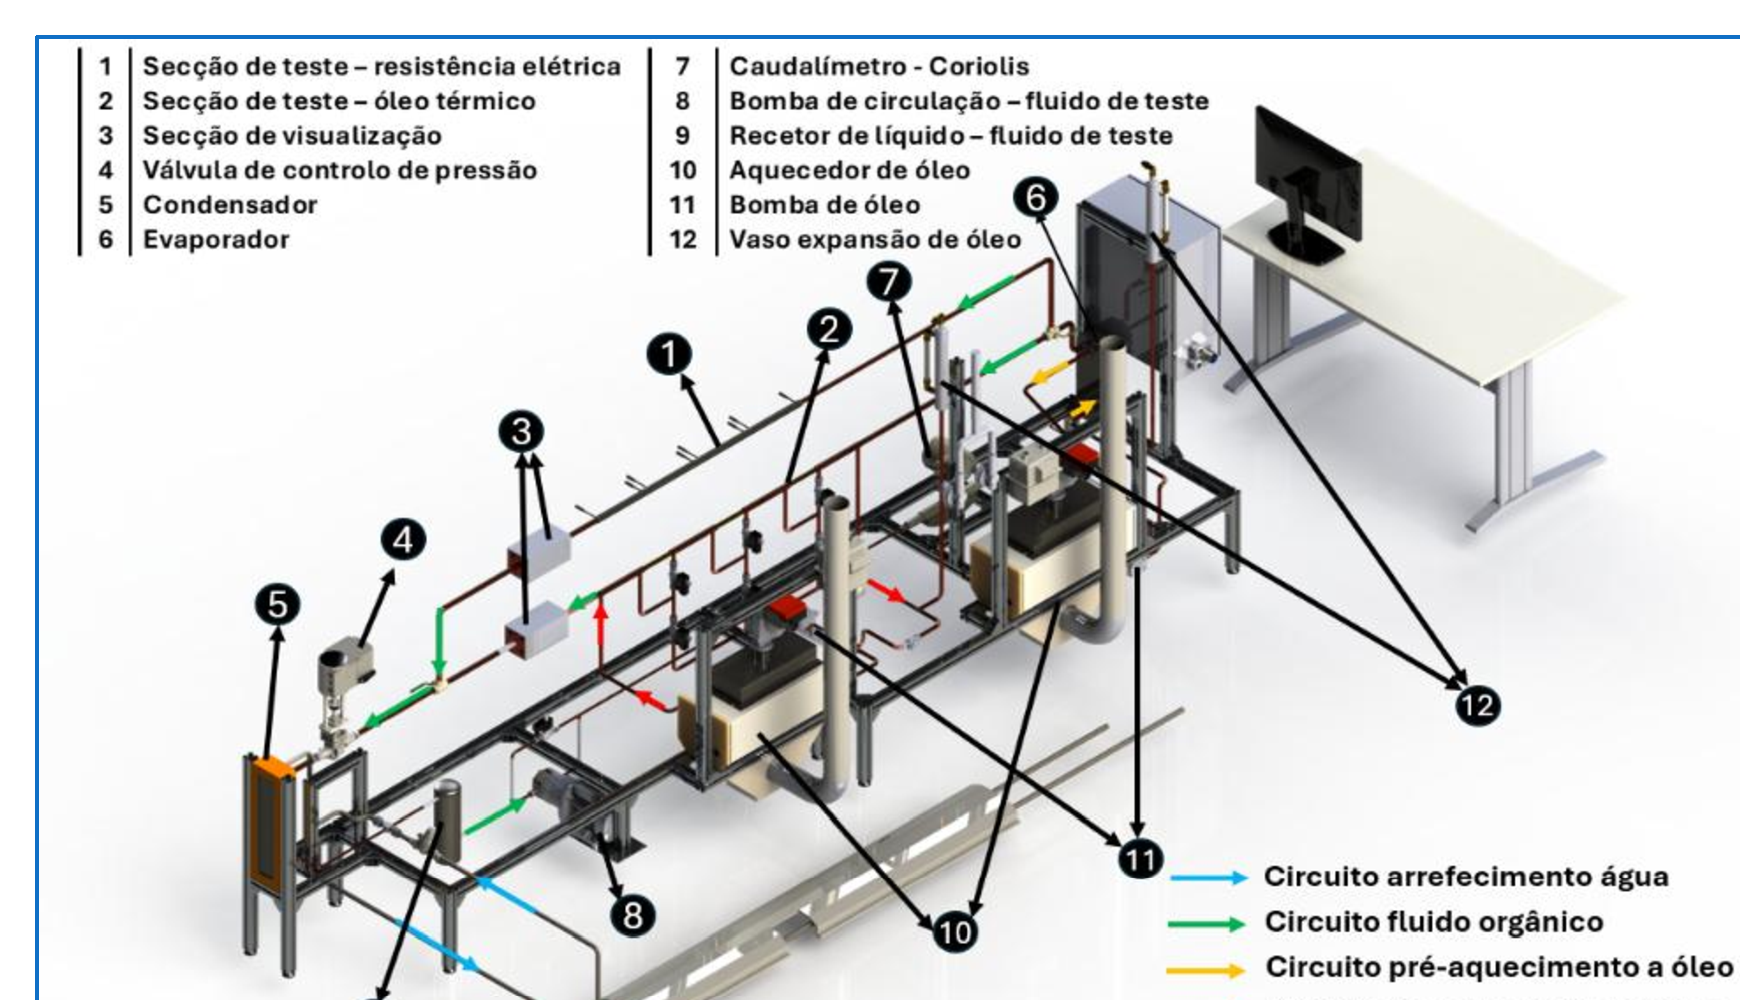
\includegraphics[width=0.92\textwidth]{assets/fig1_bancada_render.png}
    \caption{Render tridimensional da bancada experimental para estudo de escoamentos em ebulição (ADAI / UC).}
    \label{fig:bancada_render}
\end{figure}

A arquitetura geral da instalação é estruturada em torno de múltiplos subsistemas complementares:
\begin{itemize}
    \item \textbf{Circuito principal de escoamento do fluido de teste (verde na \autoref{fig:bancada_render}):} Condutas em aço inoxidável e cobre com diâmetros normalizados, integrando a bomba de recirculação magnética (item 8), o tanque recetor de líquido (item 9), secções de aquecimento, a secção de visualização transparente (item 3) e o condensador (item 5);
    \item \textbf{Secção de teste e aquecimento primário (itens 1 e 2):} Módulos térmicos dedicados ao fornecimento uniforme de fluxo de calor para indução de ebulição, com secção tubular aquecida por resistências elétricas calibradas e secção alimentada por permutador de óleo térmico;
    \item \textbf{Secção de visualização ótica transparente (item 3):} Tubo de vidro borossilicato de alta transparência ótica com diâmetro interno nominal $D_i = 20{,}0\,\mathrm{mm}$ e diâmetro externo $D_o = 26{,}0\,\mathrm{mm}$, permitindo a observação direta dos regimes de escoamento (bolhas dispersas, \emph{slugs}, transições anulares);
    \item \textbf{Circuito secundário de óleo de aquecimento (amarelo/vermelho na \autoref{fig:bancada_render}):} Compreende a bomba de circulação de óleo térmico (item 11), o aquecedor de óleo (item 10) e o vaso de expansão atmosférico/pressurizado (item 12), assegurando a regulação precisa da temperatura do óleo;
    \item \textbf{Circuito de arrefecimento e condensação (azul na \autoref{fig:bancada_render}):} Circuito de água de refrigeração ligado ao condensador de placas/tubular (item 5), responsável pela condensação total do vapor gerado e pelo subarrefecimento do fluido antes da sua recirculação;
    \item \textbf{Sistema de controlo de pressão e expansão:} Válvula reguladora de pressão motorizada (item 4), instalada a jusante da secção de ensaio, que atua na linha de retorno para estabilização da pressão operacional de saturação do ciclo;
    \item \textbf{Instrumentação e aquisição de dados:} Caudalímetro mássico de Coriolis de elevada precisão (item 7), transmissores de pressão diferencial e absoluta, e matrizes axiais e perimétricas de termopares tipo K conectadas a módulos compactos de aquisição National Instruments (NI).
\end{itemize}

\subsection{Modelação Tridimensional em CAD (SolidWorks\textregistered) e Integração Mecânica}
\label{subsec:cad_solidworks}

No decurso das atividades de julho de 2026, a principal intervenção técnica desenvolvida pelo autor concentrou-se na modelação tridimensional assistida por computador em SolidWorks\textregistered{}, com o objetivo de compatibilizar, atualizar e aperfeiçoar o projeto mecânico da bancada experimental perante novas necessidades operacionais e instrumentais da equipa de investigação.

A modelação paramétrica e a verificação tridimensional foram orientadas segundo quatro vertentes fundamentais:

\subsubsection{Integração do Tanque Recetor de Líquido (\emph{Liquid Receiver})}
\label{subsubsec:cad_liquid_receiver}

A estabilidade operacional de circuitos fechados de escoamento bifásico depende criticamente da manutenção de uma alimentação monofásica líquida estável na admissão da bomba de recirculação. A presença de bolsas de vapor arrastadas ou de oscilações bruscas de pressão pode conduzir a fenómenos severos de cavitação, degradação do caudal mássico e danos no impulsor magnético.

Por forma a mitigar estes riscos, procedeu-se à modelação e integração mecânica no modelo global em SolidWorks\textregistered{} do tanque recetor de líquido (\emph{liquid receiver}, identificado pelo item 9 na \autoref{fig:bancada_render}). O trabalho compreendeu:
\begin{enumerate}
    \item Definição do posicionamento espacial ótimo do reservatório na secção inferior da bancada, maximizando a carga hidrostática positiva disponível sobre a bomba (\emph{Net Positive Suction Head} -- NPSH);
    \item Modelação das ligações flangeadas e roscadas com as linhas de retorno de líquido arrefecido provenientes do condensador;
    \item Confeção e posicionamento de elementos de fixação mecânica estrutural aos perfis modulares de alumínio da bancada, garantindo amortecimento de vibrações e fácil acesso visual para verificação do nível de fluido.
\end{enumerate}

\subsubsection{Reconfiguração Estrutural e Elevação da Válvula Reguladora de Pressão}
\label{subsubsec:cad_valvula_pressao}

A válvula de regulação e controlo de pressão da bancada (item 4 na \autoref{fig:bancada_render}) desempenha um papel determinante na fixação do ponto termodinâmico de saturação durante os ensaios de escoamento ebulitivo. Contudo, na configuração geométrica preliminar da instalação, a válvula encontrava-se sujeita a desníveis espaciais e constrangimentos de acessibilidade para acoplamento do atuador motorizado.

O autor concebeu e modelou no SolidWorks\textregistered{} a reconfiguração estrutural do suporte da válvula:
\begin{enumerate}
    \item Modelação de uma subestrutura elevada em perfis estruturais modulares de alumínio extrudido, rigidamente acoplada à armação principal da bancada através de cantoneiras e parafusos com porca em T;
    \item Elevação geométrica da base da válvula até à cota horizontal exata das linhas de escoamento a jusante da secção de visualização, eliminando cotovelos e desvios desnecessários que geravam perdas de carga singulares indesejadas;
    \item Garantia de espaço livre circundante para manobra, instalação da cablagem de alimentação do servomotor e intervenções de manutenção periódica.
\end{enumerate}

\subsubsection{Roteamento e Alinhamento Tridimensional das Tubagens do Circuito}
\label{subsubsec:cad_tubagens}

A introdução do novo tanque recetor e a elevação da válvula de controlo exigiram a reformulação e o alinhamento das tubagens do circuito hidráulico fechado. Recorrendo às ferramentas avançadas de encaminhamento tridimensional (\emph{Routing}) do SolidWorks\textregistered{}, efetuou-se:
\begin{enumerate}
    \item Deteção e resolução de colisões e interferências geométricas (\emph{clash detection}) entre as tubagens do fluido orgânico, as linhas de óleo térmico de pré-aquecimento e as condutas de água fria do condensador;
    \item Otimização dos comprimentos lineares de tubo e garantia dos raios de curvatura mínimos admissíveis para condutas de cobre e aço inoxidável, prevenindo estrangulamentos de secção e tensões residuais mecânicas;
    \item Verificação do espaçamento perimétrico de segurança e acessibilidade ergonómica para instrumentação, sensorização perimétrica e manutenção das linhas de fluido;
    \item Posicionamento das tomadas de pressão e mangas para termopares nas zonas retilíneas a montante e a jusante dos pontos de transição, respeitando as normas de metrologia hidrodinâmica (comprimentos de desenvolvimento hidráulico mínimos $L/D \ge 10$).
\end{enumerate}

\subsubsection{Interface Mecânica e Alinhamento da Secção de Ensaio Ótica}
\label{subsubsec:cad_seccao_otica}

A preparação do desafio central de visão computacional e inteligência artificial exigiu especial atenção à secção transparente de visualização (item 3 na \autoref{fig:bancada_render}). O autor procedeu à verificação dimensional rigorosa dos apoios do tubo em vidro borossilicato ($D_i = 20{,}0\,\mathrm{mm}$), garantindo:
\begin{enumerate}
    \item Perfeito alinhamento coaxial entre as extremidades da conduta de vidro e os troços adjacentes metálicos da bancada, evitando descontinuidades de bordo ou degraus internos que pudessem induzir perturbações no escoamento ou promover pontos de nucleação espúrios antes da janela de observação;
    \item Definição do suporte estrutural livre de vibrações mecânicas para a câmara de alta velocidade e para a fonte de retroiluminação colimada com lente corretiva cilíndrica externa;
    \item Estabelecimento das dimensões espaciais exatas do campo de visão (\emph{Field of View} -- FOV), que serviram de referência física absoluta para a posterior calibração métrica pixel-a-metro desenvolvida na etapa computacional.
\end{enumerate}

\subsection{Síntese da Fase Laboratorial e de Modelação}
\label{subsec:sintese_laboratorio}

A etapa de trabalho presencial realizada em julho de 2026 permitiu consolidar a arquitetura mecânica da bancada experimental através da modelação integrada em SolidWorks\textregistered{}. A integração bem-sucedida do tanque recetor de líquido, a elevação da estrutura da válvula de pressão e o alinhamento geométrico rigoroso das tubagens e da secção ótica de ensaios asseguraram a consistência física e dimensional da instalação. 

Este trabalho de base forneceu os parâmetros geométricos determinantes (geometria interna circular de $20{,}0\,\mathrm{mm}$, alinhamento axial e características do campo de visão) indispensáveis para alimentar com rigor físico os algoritmos de segmentação semântica por inteligência artificial, reconstrução tridimensional com confinamento cordal e cinemática de alta velocidade implementados na fase subsequente em Python.

\newpage

% !TEX root = ../main.tex
\section{Trabalho Desenvolvido em Contexto Remoto (Inteligência Artificial e Visão Computacional)}
\label{sec:computacional_ia}

Durante os meses de agosto e setembro de 2026, as atividades prosseguiram em ambiente computacional avançado, com foco na conceção, implementação, treino e validação de um pipeline unificado em Python, PyTorch e OpenCV para processamento de imagem, inteligência artificial profunda e caracterização tridimensional de escoamentos ebulitivos em condutas circulares. O trabalho deu resposta integral ao desafio proposto no concurso \textbf{Capture the Future II}: \emph{<<Desenvolvimento e otimização de um algoritmo de inteligência artificial para reconhecimento e categorização de bolhas num escoamento ebulitivo>>}.

\subsection{Contexto, Desafios Óticos e Objetivos do Desafio CtF II}
\label{subsec:contexto_ia}

A caracterização física de escoamentos bifásicos por videografia de alta velocidade (\emph{High-Speed Video} -- HSV) afigura-se essencial para a compreensão dos mecanismos de nucleação, crescimento, deslizamento, coalescência e destacamento de bolhas. Contudo, em condutas circulares industriais, a extração de dados quantitativos através de visão computacional confronta-se com desafios óticos severos:
\begin{enumerate}
    \item \textbf{Efeito de lente cilíndrica do tubo:} A conduta circular em vidro borossilicato ($D_i = 20{,}0\,\mathrm{mm}$, $D_o = 26{,}0\,\mathrm{mm}$) atua como uma lente cilíndrica convergente espessa perante a retroiluminação colimada. O desfasamento dos índices de refração ($n_{\text{ar}} = 1{,}00 \to n_{\text{vidro}} \approx 1{,}50 \to n_{\text{líquido}} \approx 1{,}33$) concentra a luz numa faixa cáustica central intensa e deflete os raios próximos das paredes, gerando uma subexposição periférica acentuada junto ao bordo superior do canal --- precisamente a região para onde as bolhas e os \emph{slugs} ascendem por forças de impulsão gravítica~\cite{branco2026optical};
    \item \textbf{Reflexo ótico interno nas bolhas (\emph{glare}):} Cada bolha de vapor no seio do líquido atua como uma lente esférica divergente ($n_{\text{líquido}} \approx 1{,}33 \to n_{\text{vapor}} \approx 1{,}00$). Os raios paraxiais atravessam o núcleo gasoso sem desvio substancial, criando um ponto de luz central de intensidade idêntica à do líquido envolvente, enquanto a periferia sofre reflexão total interna originando um contorno escuro. Algoritmos clássicos de limiarização (e.g., Otsu~\cite{otsu1979threshold}) segmentam a bolha erradamente como um toro oco (artefacto de <<donut>>);
    \item \textbf{Ambiguidade de profundidade e desfoque monocular:} O registo bidimensional de uma única câmara projeta um domínio 3D com perda do eixo de visão ($z$). As bolhas fora do plano focal exibem atenuação do gradiente de intensidade na fronteira devido ao desfoque (\emph{defocus blur});
    \item \textbf{Confinamento geométrico cordal:} Na secção transversal circular, a espessura física varia verticalmente segundo o perfil de corda:
    \begin{equation}
        L_{\text{chord}}(y) = 2\sqrt{\max\left(0, \, R_{\text{pipe}}^2 - \Delta y^2\right)}
    \end{equation}
    exigindo modelos volumétricos que respeitem a curvatura real da parede e a conservação da massa.
\end{enumerate}

Para mitigar os artefactos de iluminação, a bancada integrou uma unidade LED traseira de alta intensidade combinada com uma lente cilíndrica corretiva externa especialmente projetada por traçado de raios pelo grupo de investigação~\cite{branco2026optical}, conforme esquematizado na \autoref{fig:diagrama_otica}.

\begin{figure}[!htbp]
    \centering
    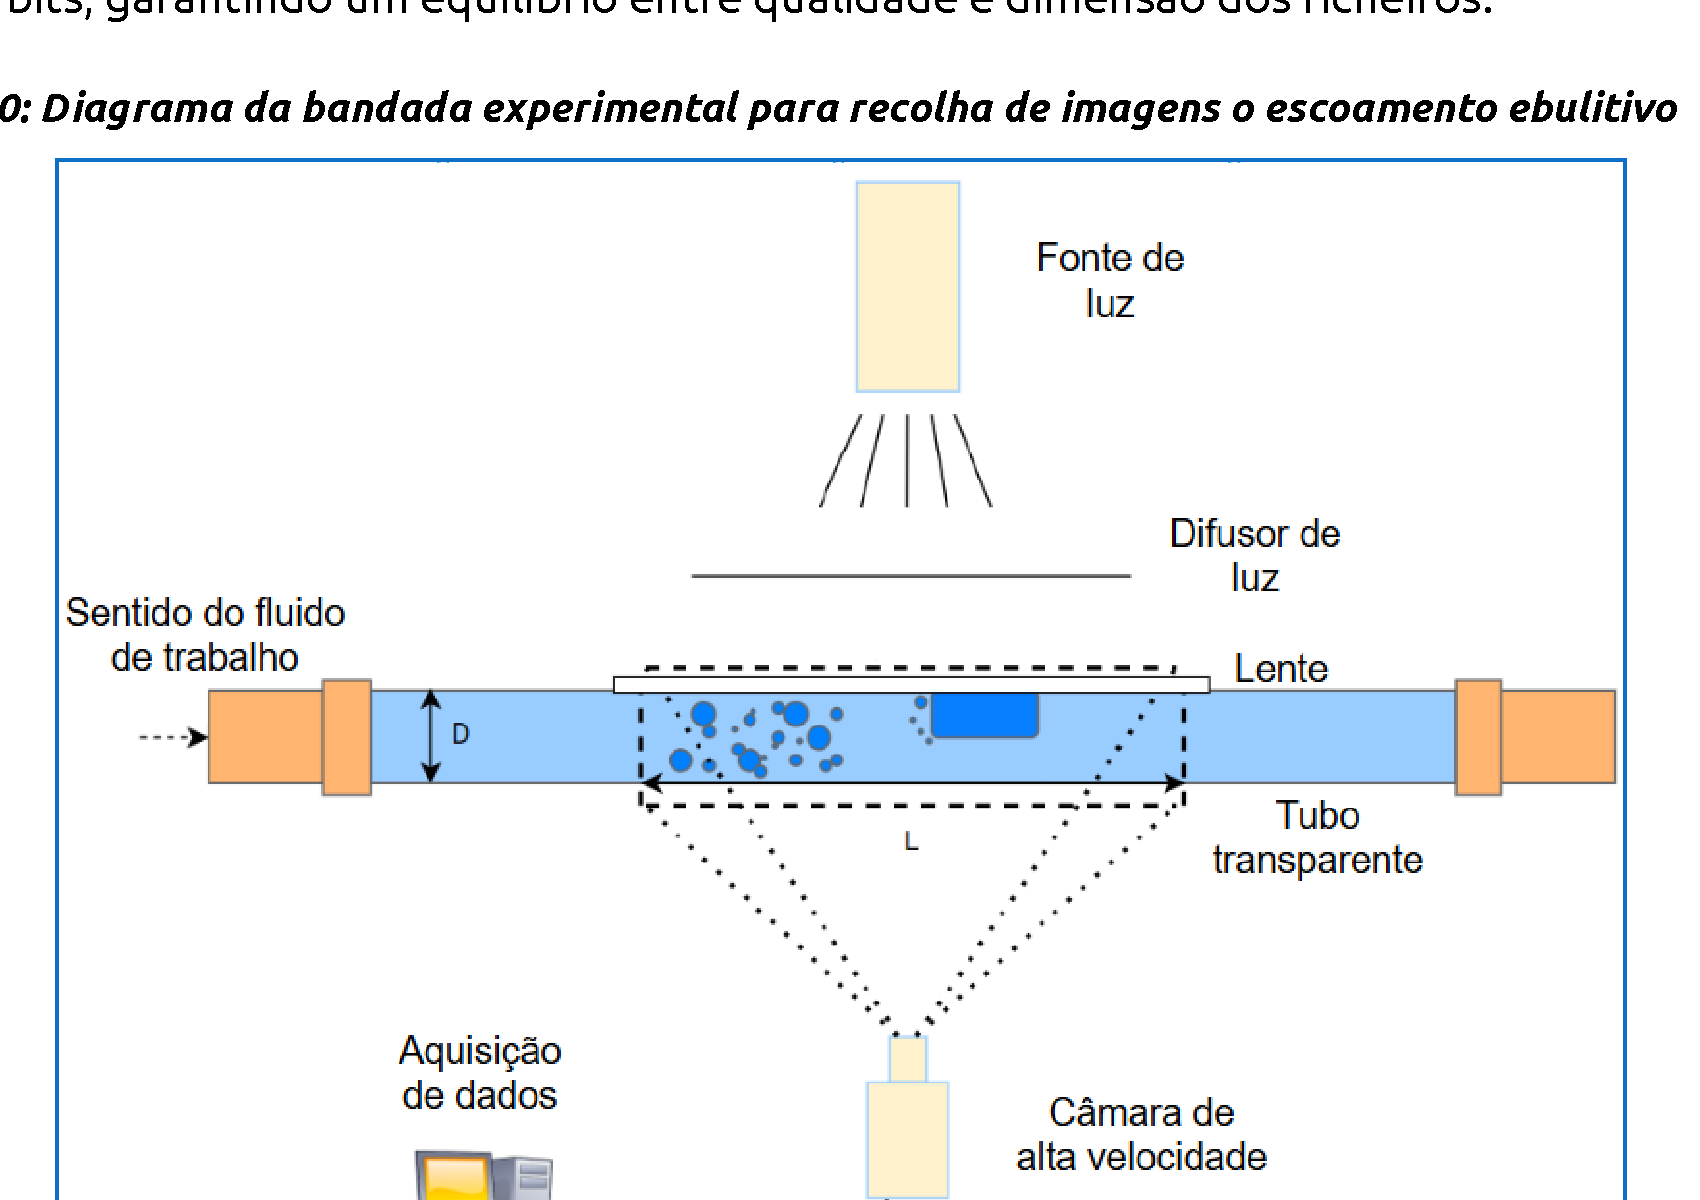
\includegraphics[width=0.85\textwidth]{assets/fig10_diagrama_otica.png}
    \caption{Diagrama esquemático da bancada ótica para aquisição de escoamentos ebulitivos com câmara de alta velocidade e iluminação traseira.}
    \label{fig:diagrama_otica}
\end{figure}

A grandeza macroscópica nuclear a quantificar é a \textbf{fração de vazio} (\emph{void fraction}, $\alpha$), definida como a fração volumétrica ocupada pela fase gasosa no volume de controlo considerado:
\begin{equation}
    \alpha = \frac{V_g}{V_g + V_l} = \frac{V_g}{V_{\text{tubo}}}
    \label{eq:void_fraction_def}
\end{equation}
sendo $V_g$ o volume total tridimensional de gás e $V_{\text{tubo}} = \pi R_{\text{pipe}}^2 W_{\text{FOV}}$ o volume interno da secção cilíndrica monitorizada no campo de visão (\emph{Field of View} -- FOV).

\subsection{Estado da Arte e Inovação da Nova Arquitetura em Python}
\label{subsec:estado_da_arte_ia}

Nos últimos anos, a aplicação de redes neuronais convolucionais baseadas na arquitetura U-Net~\cite{ronneberger2015unet} revolucionou a análise de bolhas em escoamentos térmicos. Seong et al.~\cite{seong2023automated} (MIT) aplicaram uma U-Net clássica com \emph{transfer learning} a bolhas em ebulição subarrefecida em placas planas a 10\,000~FPS, combinando-a com fluxo ótico global de Horn--Schunck~\cite{hornschunck1981}. Passoni et al.~\cite{passoni2024integrating} utilizaram redes convolucionais para estimar a fração de vazio em canais corrugados. Numa abordagem preliminar desenvolvida anteriormente no projeto em MATLAB, utilizou-se uma U-Net otimizada por \emph{Particle Swarm Optimization} (PSO)~\cite{kennedy1995particle}. Contudo, essa implementação inicial apresentava limitações metodológicas e operacionais relevantes:
\begin{itemize}
    \item Dependência do ambiente proprietário MATLAB, com reduzida escalabilidade para processamento em lote e integração de modelos estado-da-arte de visão computacional;
    \item Ausência de conexões residuais no codificador, provocando lentidão na convergência e suscetibilidade à degradação de gradientes durante o \emph{backpropagation};
    \item Utilização exclusiva de funções de perda baseadas em entropia cruzada clássica, vulneráveis ao extremo desequilíbrio entre classes (líquido $>95\%$ da imagem vs. microbolhas gasosas $<5\%$), gerando uma elevada taxa de falsos negativos;
    \item Erro dimensional na formulação da reconstrução volumétrica elipsoidal, onde o semi-eixo de profundidade fora erroneamente definido como a corda total $2\sqrt{R^2-\Delta y^2}$ em vez do semi-eixo de raio $\sqrt{R^2-\Delta y^2}$, introduzindo uma sobrestimação de 100\% no volume das bolhas esferoidais;
    \item Rastreamento cinemático dependente de vizinhos mais próximos gulosos (\emph{greedy}), que colapsava perante rotações, deformações bruscas e eventos de quebra hidrodinâmica (\emph{breakup});
    \item Inexistência de estimativa da coordenada de profundidade fora do plano ($z$).
\end{itemize}

Para superar definitivamente estas restrições, desenvolveu-se em 2026 um ecossistema modular inteiramente em Python, com orquestração centralizada via CLI em \texttt{main.py}. Na \autoref{tab:comparacao_tecnica} sumariza-se o salto qualitativo da nossa abordagem face à literatura e aos scripts exploratórios preliminares em MATLAB desenvolvidos anteriormente no projeto.

\begin{table}[!htbp]
\centering
\small
\caption{Comparação técnica entre abordagens da literatura, baseline preliminar em MATLAB e a nova implementação em Python (2026).}
\label{tab:comparacao_tecnica}
\begin{tabularx}{\textwidth}{>{\raggedright\arraybackslash}p{3.2cm}>{\raggedright\arraybackslash}X>{\raggedright\arraybackslash}X>{\raggedright\arraybackslash}X}
\toprule
\textbf{Característica} & \textbf{Seong et al. (MIT, 2023)} & \textbf{Baseline Preliminar (MATLAB)} & \textbf{Nossa Implementação 2026 (Python)} \\
\midrule
Ambiente \& Framework & Python / TensorFlow & MATLAB Deep Learning & Python 3.12 / PyTorch / OpenCV \\
Codificador (Backbone) & U-Net Clássica (2015) & U-Net Clássica com PSO & \textbf{ResNet-34 Residual (Pré-treinada ImageNet)} \\
Função de Perda & Cross-Entropy pura & Cross-Entropy pura & \textbf{Híbrida: BCE + Dice Loss balanceada} \\
Anotação \& Glare & Contraste básico & Limiarização binarizada & \textbf{Polígonos sólidos (\texttt{fillPoly}), zero donuts} \\
Reconstrução 3D & Área projetada 2D & Extrusão com erro cordal & \textbf{Duplo regime SI ($\mathrm{m}^3$) com confinamento cordal} \\
Rastreio Cinemático & Fluxo Ótico Global & Vizinho Próximo guloso & \textbf{Kuhn--Munkres Húngaro + Quarentena Breakup} \\
Eixo de Profundidade & Inexistente (Plano 2D) & Inexistente (Plano 2D) & \textbf{Depth from Defocus (DFD) com Smoothstep $C^1$} \\
\bottomrule
\end{tabularx}
\end{table}

\subsection{Treino da Rede Neuronal e Otimização}
\label{subsec:treino_unet}

\subsubsection{Arquitetura ResNet-34 U-Net e Função de Perda Híbrida}
\label{subsubsec:unet_arch_loss}

A rede neuronal desenvolvida e treinada neste trabalho baseia-se na arquitetura U-Net~\cite{ronneberger2015unet} dotada de um codificador pré-treinado no repositório ImageNet com blocos residuais de ResNet-34~\cite{he2016deep}, esquematizada na \autoref{fig:unet_arch}. Os blocos residuais com conexões de salto direto (\emph{skip connections}) minoram a degradação de gradientes durante o \emph{backpropagation}, permitindo uma aprendizagem estável e acelerada com convergência rápida mesmo a partir de uma base contendo poucas dezenas de imagens com anotação manual fidedigna ($N \approx 20\text{--}30$ fotogramas representativos gerados via Label Studio com polígonos fechados \texttt{cv2.fillPoly}).

\begin{figure}[!htbp]
    \centering
    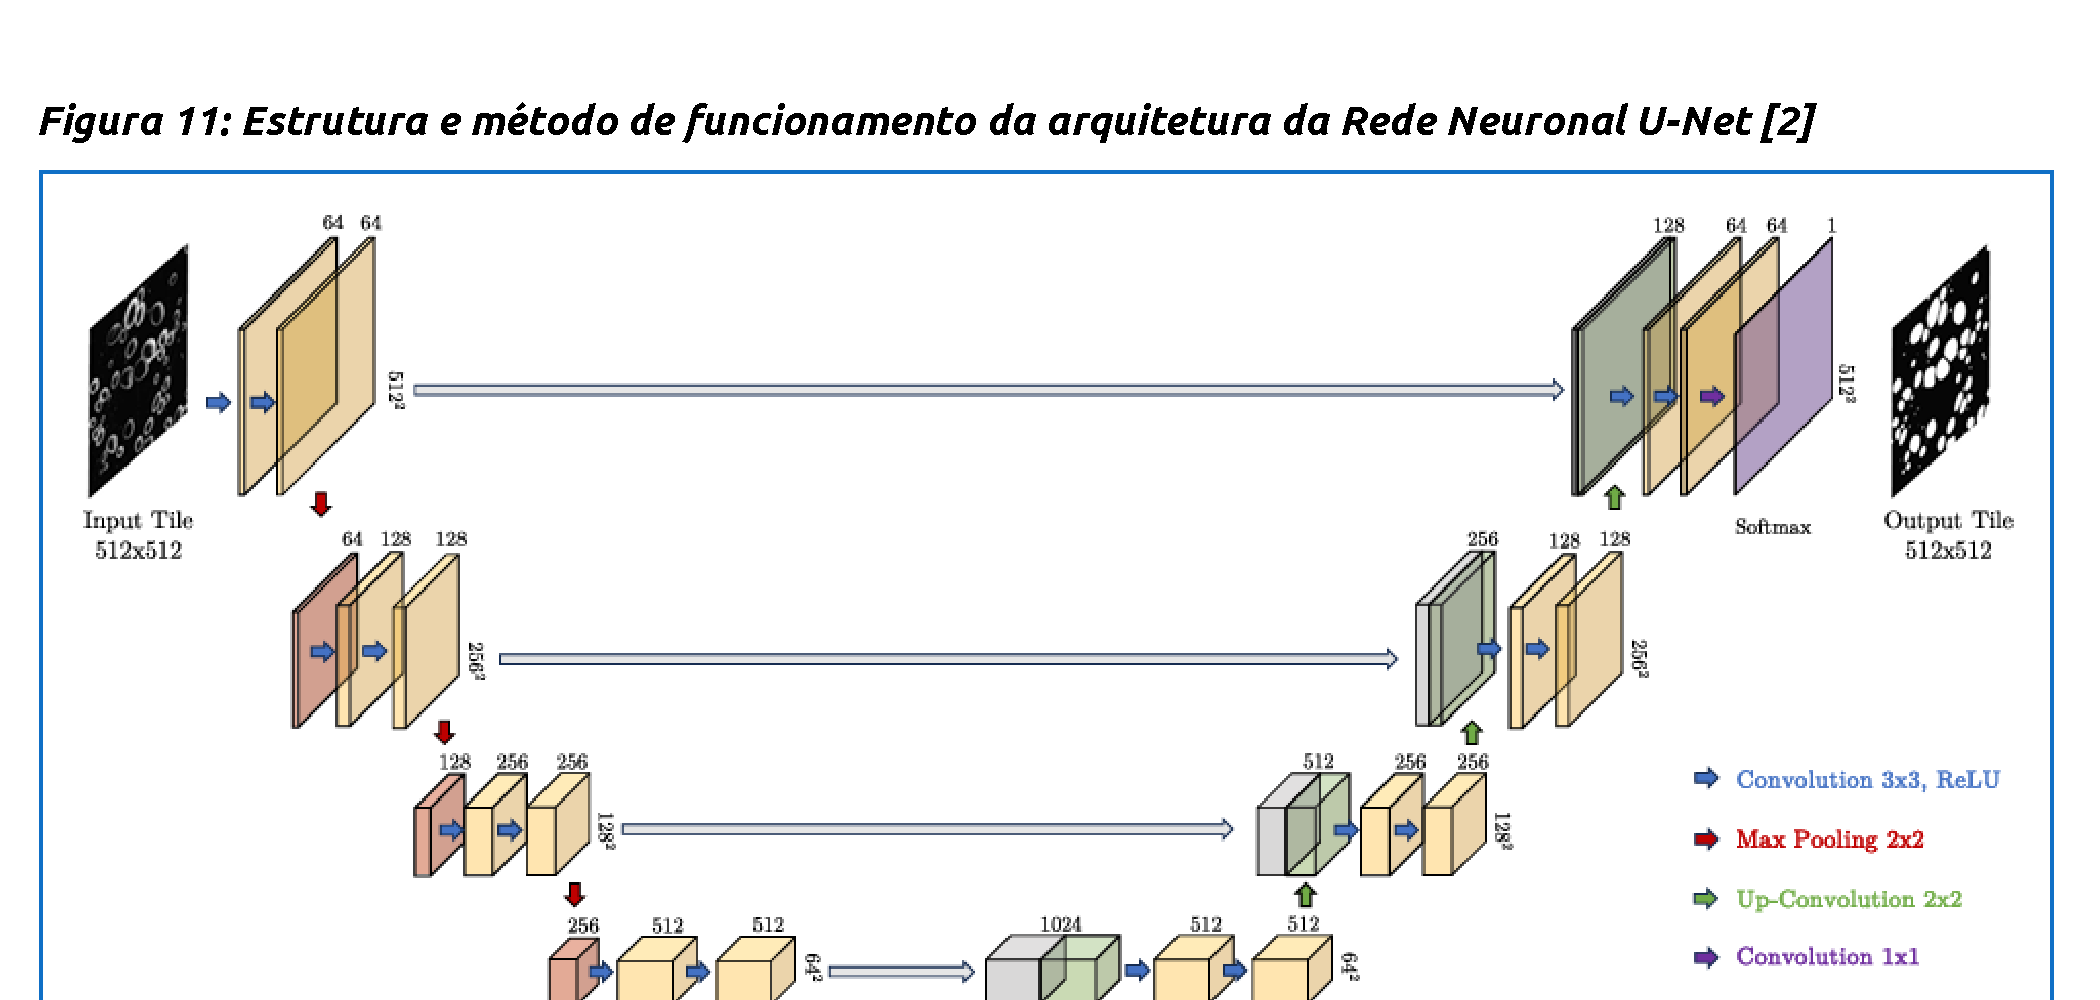
\includegraphics[width=0.92\textwidth]{assets/fig11_unet_arch.png}
    \caption{Arquitetura da rede ResNet-34 U-Net com conexões residuais e perda híbrida para segmentação de bolhas.}
    \label{fig:unet_arch}
\end{figure}

Para mitigar o severo desequilíbrio entre classes típico de regimes ebulitivos dispersos (onde a fase líquida contínua preenche tipicamente mais de 90\% do domínio visual e as microbolhas de vapor representam apenas uma pequena fração dos píxeis), concebeu-se uma função de perda híbrida combinando a Entropia Cruzada Binária ($\mathcal{L}_{\text{BCE}}$) e o Coeficiente de Sobreposição de Dice ($\mathcal{L}_{\text{Dice}}$)~\cite{milletari2016vnet}:
\begin{equation}
    \mathcal{L}_{\text{total}} = \mathcal{L}_{\text{BCE}}(y, \hat{y}) + \mathcal{L}_{\text{Dice}}(y, \hat{y})
    \label{eq:hybrid_loss}
\end{equation}
\begin{equation}
    \mathcal{L}_{\text{BCE}} = -\frac{1}{N_{\text{pix}}} \sum_{p=1}^{N_{\text{pix}}} \left[ y_p \log(\hat{y}_p) + (1 - y_p) \log(1 - \hat{y}_p) \right]
\end{equation}
\begin{equation}
    \mathcal{L}_{\text{Dice}} = 1 - \frac{2 \sum_{p=1}^{N_{\text{pix}}} y_p \hat{y}_p + \epsilon_{\text{smooth}}}{\sum_{p=1}^{N_{\text{pix}}} y_p + \sum_{p=1}^{N_{\text{pix}}} \hat{y}_p + \epsilon_{\text{smooth}}}
\end{equation}
onde $y_p \in \{0, 1\}$ é a máscara real anotada, $\hat{y}_p = \sigma(z_p) \in [0, 1]$ representa a probabilidade sigmoid predita e $\epsilon_{\text{smooth}} = 1{,}0$ denota o termo de regularização suave de Laplace. Ao avaliar a interceção espacial entre as entidades gasosas, a parcela de Dice penaliza fortemente falsos negativos sem permitir que a vasta predominância de verdadeiros negativos na fase líquida mascare a eficácia do modelo.

\subsubsection{Estratégia de Treino e Otimização Hiperparamétrica}
\label{subsubsec:training_strategy}

A otimização dos pesos neuronais foi governada pelo algoritmo AdamW com taxa de aprendizagem inicial de $\eta_0 = 10^{-4}$, decaimento de peso $\lambda_{\text{weight}} = 10^{-2}$ e escalonamento por agendamento de cosseno amortecido (\emph{Cosine Annealing Learning Rate}). Com vista a prevenir a sobremororização (\emph{overfitting}) e dotar a rede de invariância a reflexos luminescentes parasitas, empregou-se uma rotina avançada de aumento artificial de dados (\emph{data augmentation}) através da biblioteca Albumentations: rotações angulares aleatórias ($\pm 15^\circ$), inversões especulares horizontais e verticais, modulações subtis de gama e contraste ($\pm 10\%$) simulando oscilações térmicas da lâmpada halogénea e adição controlada de ruído gaussiano. O procedimento de treino atingiu a convergência ótima ao fim de 40 épocas, ativando o mecanismo de paragem antecipada com base no índice IoU de validação.

\subsubsection{Validação do Modelo, Métricas de Desempenho e Matriz de Confusão}
\label{subsubsec:validation_metrics}

A quantificação do poder preditivo do modelo foi efetuada através do módulo \nolinkurl{evaluate_unet_metrics.py} sobre um conjunto de teste totalmente segregado do treino. Os parâmetros globais de desempenho são discriminados na \autoref{tab:metricas_unet}.

\begin{table}[!htbp]
\centering
\small
\caption{Métricas de desempenho da rede ResNet-34 U-Net no conjunto de teste independente.}
\label{tab:metricas_unet}
\begin{tabularx}{\textwidth}{lcr>{\raggedright\arraybackslash}X}
\toprule
\textbf{Métrica de Avaliação} & \textbf{Valor Absoluto} & \textbf{Percentagem} & \textbf{Significado Físico / Algorítmico} \\
\midrule
Exatidão (\emph{Accuracy}) & $0{,}9499$ & $94{,}99\%$ & Proporção global de píxeis corretamente previstos \\
Precisão (\emph{Precision}) & $0{,}9794$ & $97{,}94\%$ & Pureza das predições gasosas (reduzidos falsos positivos) \\
Sensibilidade (\emph{Recall}) & $0{,}9025$ & $90{,}25\%$ & Capacidade de identificar a totalidade das bolhas reais \\
Especificidade (\emph{Specificity}) & $0{,}9857$ & $98{,}57\%$ & Rigor na classificação da fase líquida contínua \\
\textbf{F1-Score / Coeficiente Dice} & $\mathbf{0{,}9394}$ & $\mathbf{93{,}94\%}$ & Média harmónica entre Precisão e Sensibilidade \\
\textbf{Índice de Jaccard (IoU)} & $\mathbf{0{,}8857}$ & $\mathbf{88{,}57\%}$ & Grau de sobreposição espacial direta entre conjuntos \\
Coeficiente de Matthews (MCC) & $0{,}8990$ & $0{,}8990$ & Correlação balanceada entre classes (escala $-1$ a $+1$) \\
\midrule
Verdadeiros Positivos ($TP$) & \multicolumn{2}{c}{$340\,267$ píxeis} & Fase gasosa corretamente classificada \\
Verdadeiros Negativos ($TN$) & \multicolumn{2}{c}{$492\,551$ píxeis} & Fase líquida corretamente classificada \\
Falsos Positivos ($FP$) & \multicolumn{2}{c}{$7\,159$ píxeis} & Fundo classificado erradamente como bolha \\
Falsos Negativos ($FN$) & \multicolumn{2}{c}{$36\,767$ píxeis} & Regiões de bolha omitidas pelo modelo \\
\bottomrule
\end{tabularx}
\end{table}

Na \autoref{fig:segmentation_comparison} apresenta-se um exemplo de segmentação, onde se comprova que mesmo sob presença de reflexos óticos internos e causticas no vidro, a rede prevê contornos fechados, nítidos e consistentes.

\begin{figure}[!htbp]
    \centering
    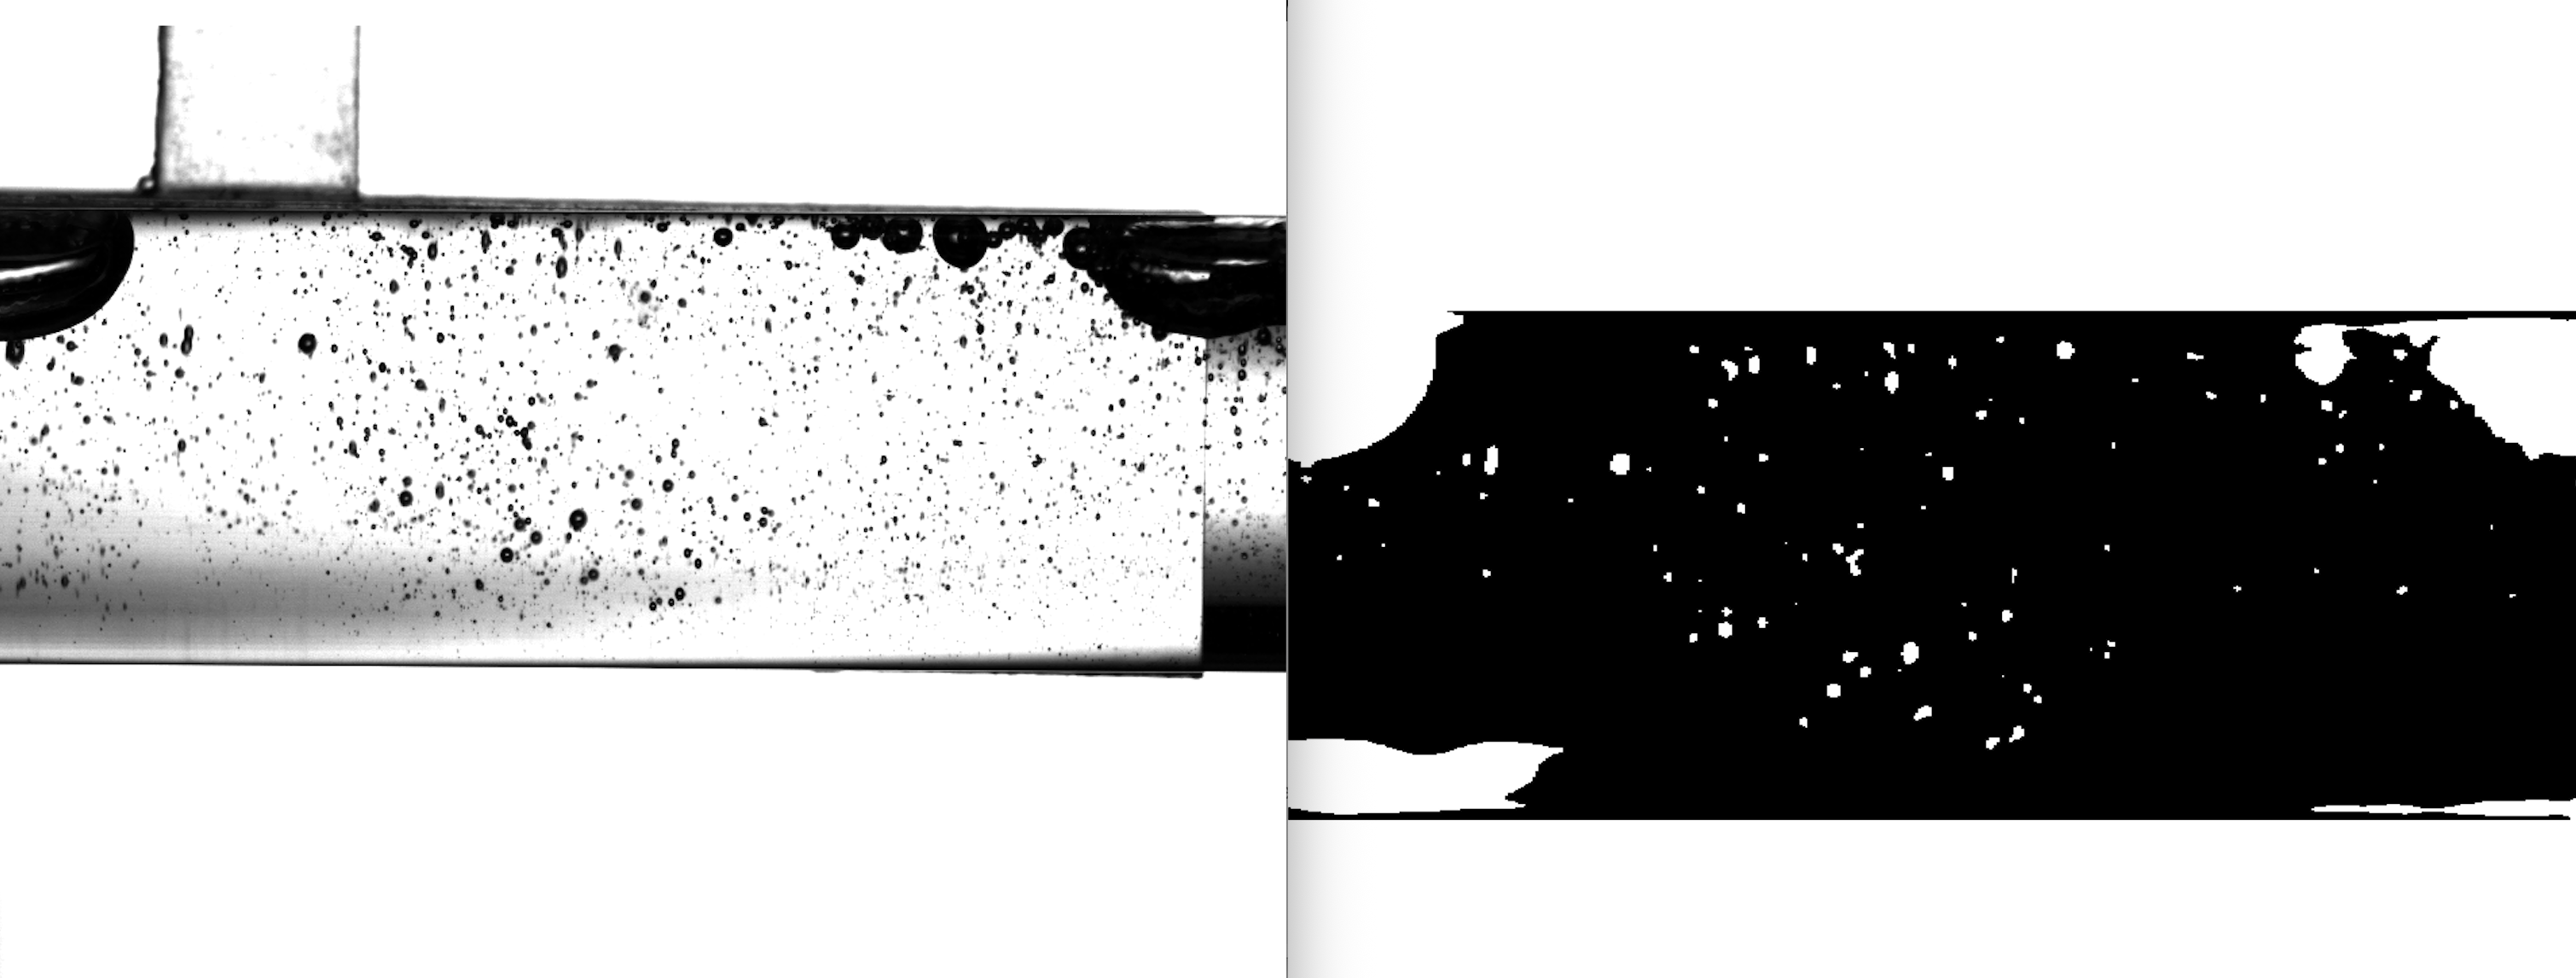
\includegraphics[width=0.92\textwidth]{assets/fig_segmentation_comparison.png}
    \caption{Comparação direta entre o fotograma experimental bruto em tons de cinzento (esquerda) e a máscara binária sólida gerada pelo modelo ResNet-34 U-Net (direita).}
    \label{fig:segmentation_comparison}
\end{figure}

\subsection{Reconstrução Volumétrica Tridimensional de Duplo Regime}
\label{subsec:reconstrucao_3d}

\subsubsection{Pré-Processamento Ótico, Calibração Métrica e Subtração de Fundo}
\label{subsubsec:pre_processing}

A determinação volumétrica fidedigna parte do isolamento da secção interior útil do canal com recurso ao script \nolinkurl{roi_crop_pre_processing.py}, suprimindo reflexos exteriores e fixações mecânicas. 

A calibração dimensional entre píxeis e grandezas físicas no Sistema Internacional é executada pelo utilitário \nolinkurl{test_calibration.py}. A partir do diâmetro interior nominal da secção transparente ($D_i = 20{,}0\,\mathrm{mm}$), estabeleceu-se a escala espacial rigorosa de $s_{\text{px}} = 8{,}60 \times 10^{-5}\,\mathrm{m/px}$ ($86{,}0\,\mu\mathrm{m/pixel}$) para a campanha de alta velocidade analisada. O procedimento de calibração métrica e deteção de interfaces é demonstrado na \autoref{fig:calibracao_pixel}.

\begin{figure}[!htbp]
    \centering
    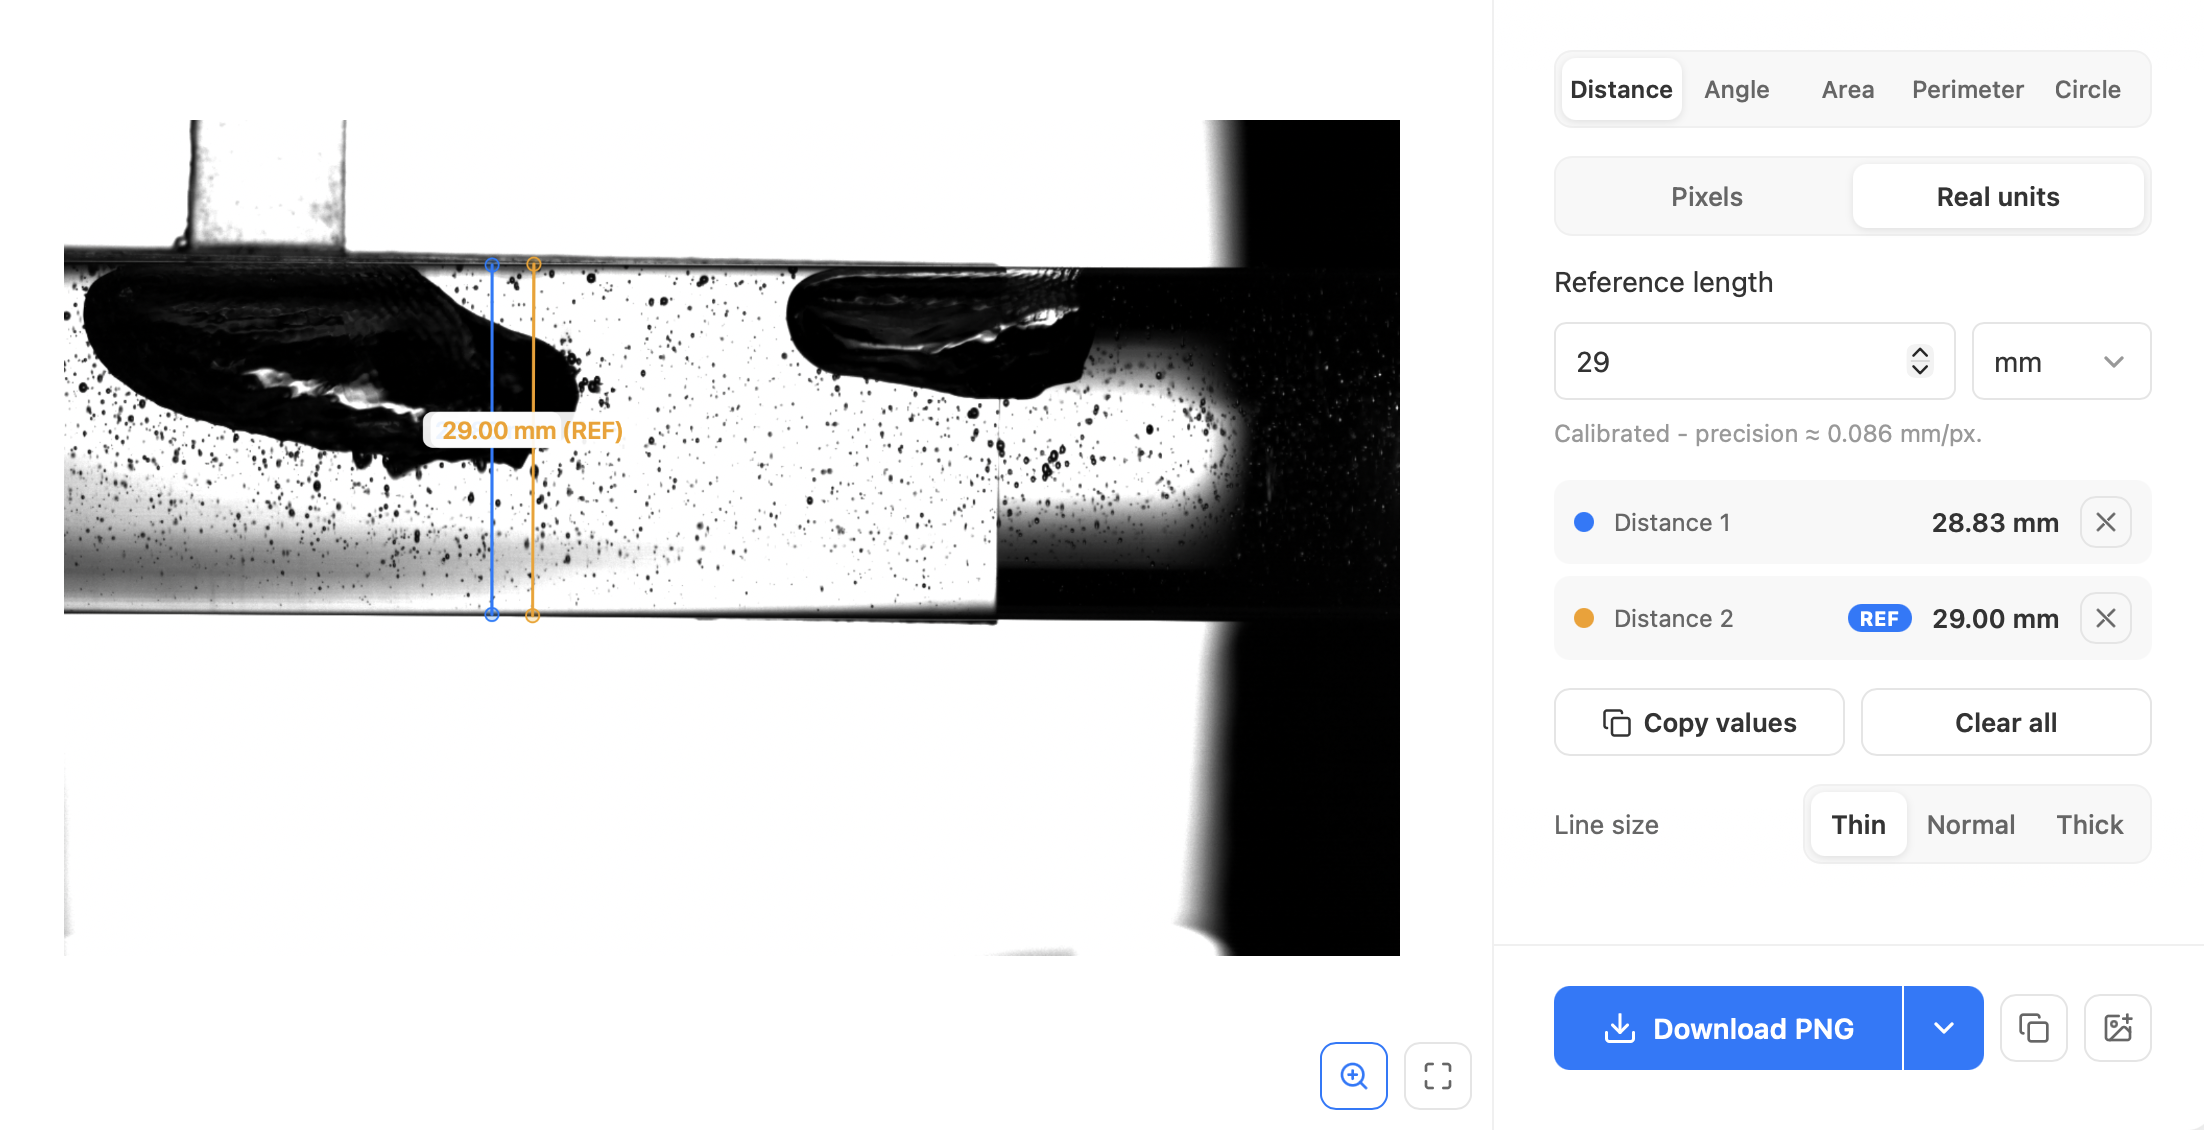
\includegraphics[width=0.88\textwidth]{assets/fig_calibracao_pixel.png}
    \caption{Interface de calibração métrica entre o diâmetro físico do canal ($20{,}0\,\mathrm{mm}$) e a resolução em píxeis.}
    \label{fig:calibracao_pixel}
\end{figure}

De modo a viabilizar a extração precisa de perfis de intensidade e desfoque, implementou-se em \nolinkurl{image_scripts/0_background_subtraction.py} uma rotina de subtração de fundo assente na aquisição de uma imagem de referência monofásica de líquido puro $I_{\text{bg}}(x, y)$, obtida sob idêntica pressão e caudal:
\begin{equation}
    I_{\text{diff}}(x, y) = \max\left(0, \, I_{\text{bg}}(x, y) - I_{\text{raw}}(x, y)\right)
\end{equation}
\begin{equation}
    I_{\text{norm}}(x, y) = \frac{I_{\text{diff}}(x, y)}{\max_{(x,y)} I_{\text{diff}}(x, y) + \varepsilon}
\end{equation}
mantendo-se uma margem de proteção morfológica de 5 píxeis em torno das fronteiras para preservar os gradientes interfaciais. Investigou-se e refutou-se a hipótese de sintetizar o fundo por mediana temporal, uma vez que em regimes de ebulição com escoamento horizontal os grandes \emph{slugs} residem permanentemente na geratriz superior da conduta devido ao empuxo, o que conduziria à inclusão indevida de sombras de vapor no fundo estático gerado.

\subsubsection{Regime 1: Bolhas Pequenas e Elipsoides Confinados}
\label{subsubsec:regime1_bolhas}

A passagem de silhuetas 2D a volumes tridimensionais físicos ($V_g$) assenta num modelo de duplo regime governado pela área de transição $A_{\text{thresh}} = \pi R_{\text{pipe}}^2$.

Para bolhas dispersas de diâmetro inferior ao raio do canal ($A_{\text{proj}} < A_{\text{thresh}}$), assume-se a geometria de elipsoides triaxiais $(a, b, c)$. Os semi-eixos no plano de visualização $xy$ ($a$ e $b$) são determinados por ajuste algébrico direto de mínimos quadrados segundo Fitzgibbon et al.~\cite{fitzgibbon1999direct}. Nos casos em que irregularidades morfológicas induzem sobrestimação de $\pi a b$, aplica-se um fator de escala de conservação estrita de área:
\begin{equation}
    \gamma = \min\left(1{,}0, \, \sqrt{\frac{A_{\text{proj}}}{\pi a b}}\right), \qquad a \leftarrow \gamma \cdot a, \quad b \leftarrow \gamma \cdot b
\end{equation}

O semi-eixo de profundidade ($c$) ao longo do eixo de visão é restringido pela geometria cilíndrica da conduta à coordenada transversal vertical $y_c$:
\begin{equation}
    c = \min\left(b, \, c_{\max}(y_c)\right) = \min\left(b, \, \sqrt{R_{\text{pipe}}^2 - (y_c - y_0)^2}\right)
\end{equation}
resultando no volume elipsoidal:
\begin{equation}
    V_{\text{small}, i} = \frac{4}{3} \pi a b c
\end{equation}
Esta formulação corrige o erro dimensional verificado nos scripts exploratórios preliminares em MATLAB (nos quais constava $c = 2\sqrt{R^2-\Delta y^2}$), prevenindo qualquer violação física da parede sólida do tubo. A \autoref{fig:reconstrucao_frame16} ilustra a correspondência entre a imagem 2D e os elipsoides 3D reconstituídos.

\begin{figure}[!htbp]
    \centering
    \begin{subfigure}[b]{0.48\textwidth}
        \centering
        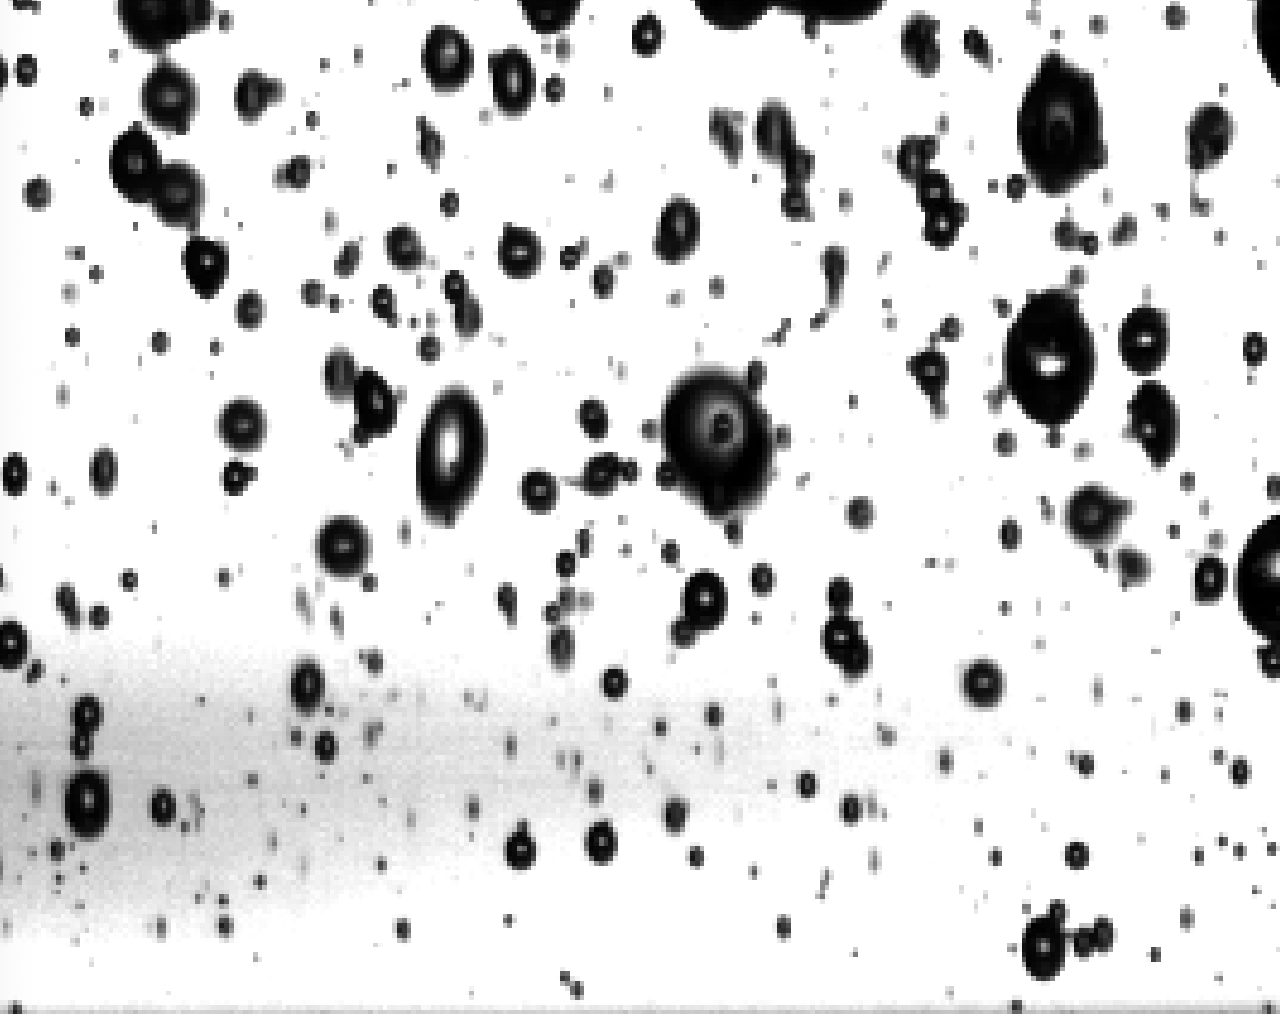
\includegraphics[width=\linewidth]{assets/fig_frame16_2d.png}
        \caption{Projeção 2D de alta velocidade.}
        \label{fig:frame16_2d}
    \end{subfigure}
    \hspace{0.02\textwidth}
    \begin{subfigure}[b]{0.48\textwidth}
        \centering
        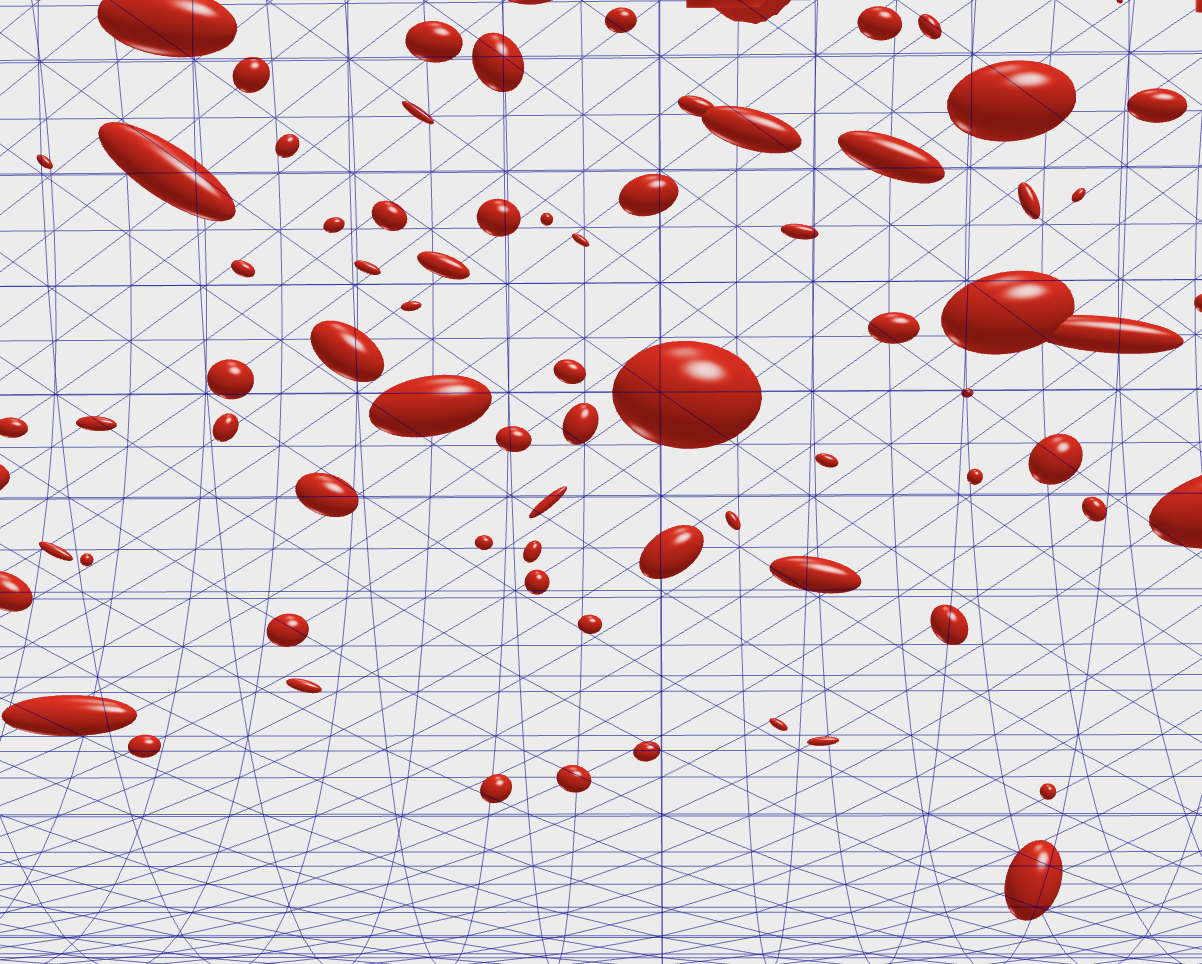
\includegraphics[width=\linewidth]{assets/fig_frame16_3d.png}
        \caption{Reconstrução elipsoidal 3D cordal.}
        \label{fig:frame16_3d}
    \end{subfigure}
    \caption{Visualização comparativa da reconstrução tridimensional no Regime 1 (bolhas pequenas dispersas sob confinamento cordal).}
    \label{fig:reconstrucao_frame16}
\end{figure}

\subsubsection{Regime 2: Grandes Slugs Deformados e Extrusão Bounded por EDT}
\label{subsubsec:regime2_slugs}

Para bolhas de grandes dimensões ou \emph{slugs} ($A_{\text{proj}} \ge A_{\text{thresh}}$) com deformação substancial ao longo da geratriz do tubo, aplica-se a Transformada de Distância Euclidiana (EDT)~\cite{felzenszwalb2012distance} $d_{\text{phys}}(p) = d(p) \cdot s_{\text{px}}$ sobre a máscara binária interior $\Omega_{\text{slug}}$. O perfil de espessura de extrusão $D'(p)$ é limitado pela corda cilíndrica geométrica local $L_{\text{chord}}(y)$:
\begin{equation}
    D'(p) = L_{\text{chord}}(y) \cdot \exp\left(-\frac{1}{\lambda_{\text{phys}} d_{\text{phys}}(p) + \varepsilon}\right)
\end{equation}
\begin{equation}
    D_{\text{bounded}}(p) = \min\left(D'(p), \, L_{\text{chord}}(y)\right)
\end{equation}
onde $\lambda_{\text{phys}} = \lambda_{\text{px}} / s_{\text{px}} \approx 1{,}7 \times 10^3\,\mathrm{m}^{-1}$ (calibrado a partir de $\lambda_{\text{px}} = 0{,}15\,\mathrm{px}^{-1}$ no modelo auditado). O volume é computado por integração de superfície em unidades SI ($\mathrm{m}^3$):
\begin{equation}
    V_{\text{slug}, i} = s_{\text{px}}^2 \sum_{p \in \Omega_i} D_{\text{bounded}}(p)
\end{equation}

\subsubsection{Cálculo da Fração de Vazio no Volume de Controlo}
\label{subsubsec:void_fraction_calc}

A fração de vazio instantânea $\alpha(t)$ é avaliada com rigor físico em cada instante integrando a totalidade dos volumes gasosos de ambos os regimes no interior do volume de controlo cilíndrico $V_{\text{tubo}} = \pi R_{\text{pipe}}^2 W_{\text{FOV}}$, conforme definido na \autoref{eq:void_fraction_def}. A implementação em unidades estritamente coerentes do Sistema Internacional previne discrepâncias de escala entre fotogramas e diferentes resoluções óticas.

\subsubsection{Visualização Tridimensional e Renderização do Escoamento}
\label{subsubsec:visualizacao_3d}

Para além do cálculo quantitativo, o algoritmo integra rotinas de renderização fotorrealista com malhas 3D texturizadas e mapas de densidade volumétrica. Na \autoref{fig:reconstrucao_3d_cilindrica} e na \autoref{fig:reconstrucao_large_slug} exibem-se as reconstituições tridimensionais geradas, evidenciando o tubo transparente, a coexistência entre bolhas dispersas e macro-slugs, e o respeito integral pelas fronteiras do canal.

\begin{figure}[!htbp]
    \centering
    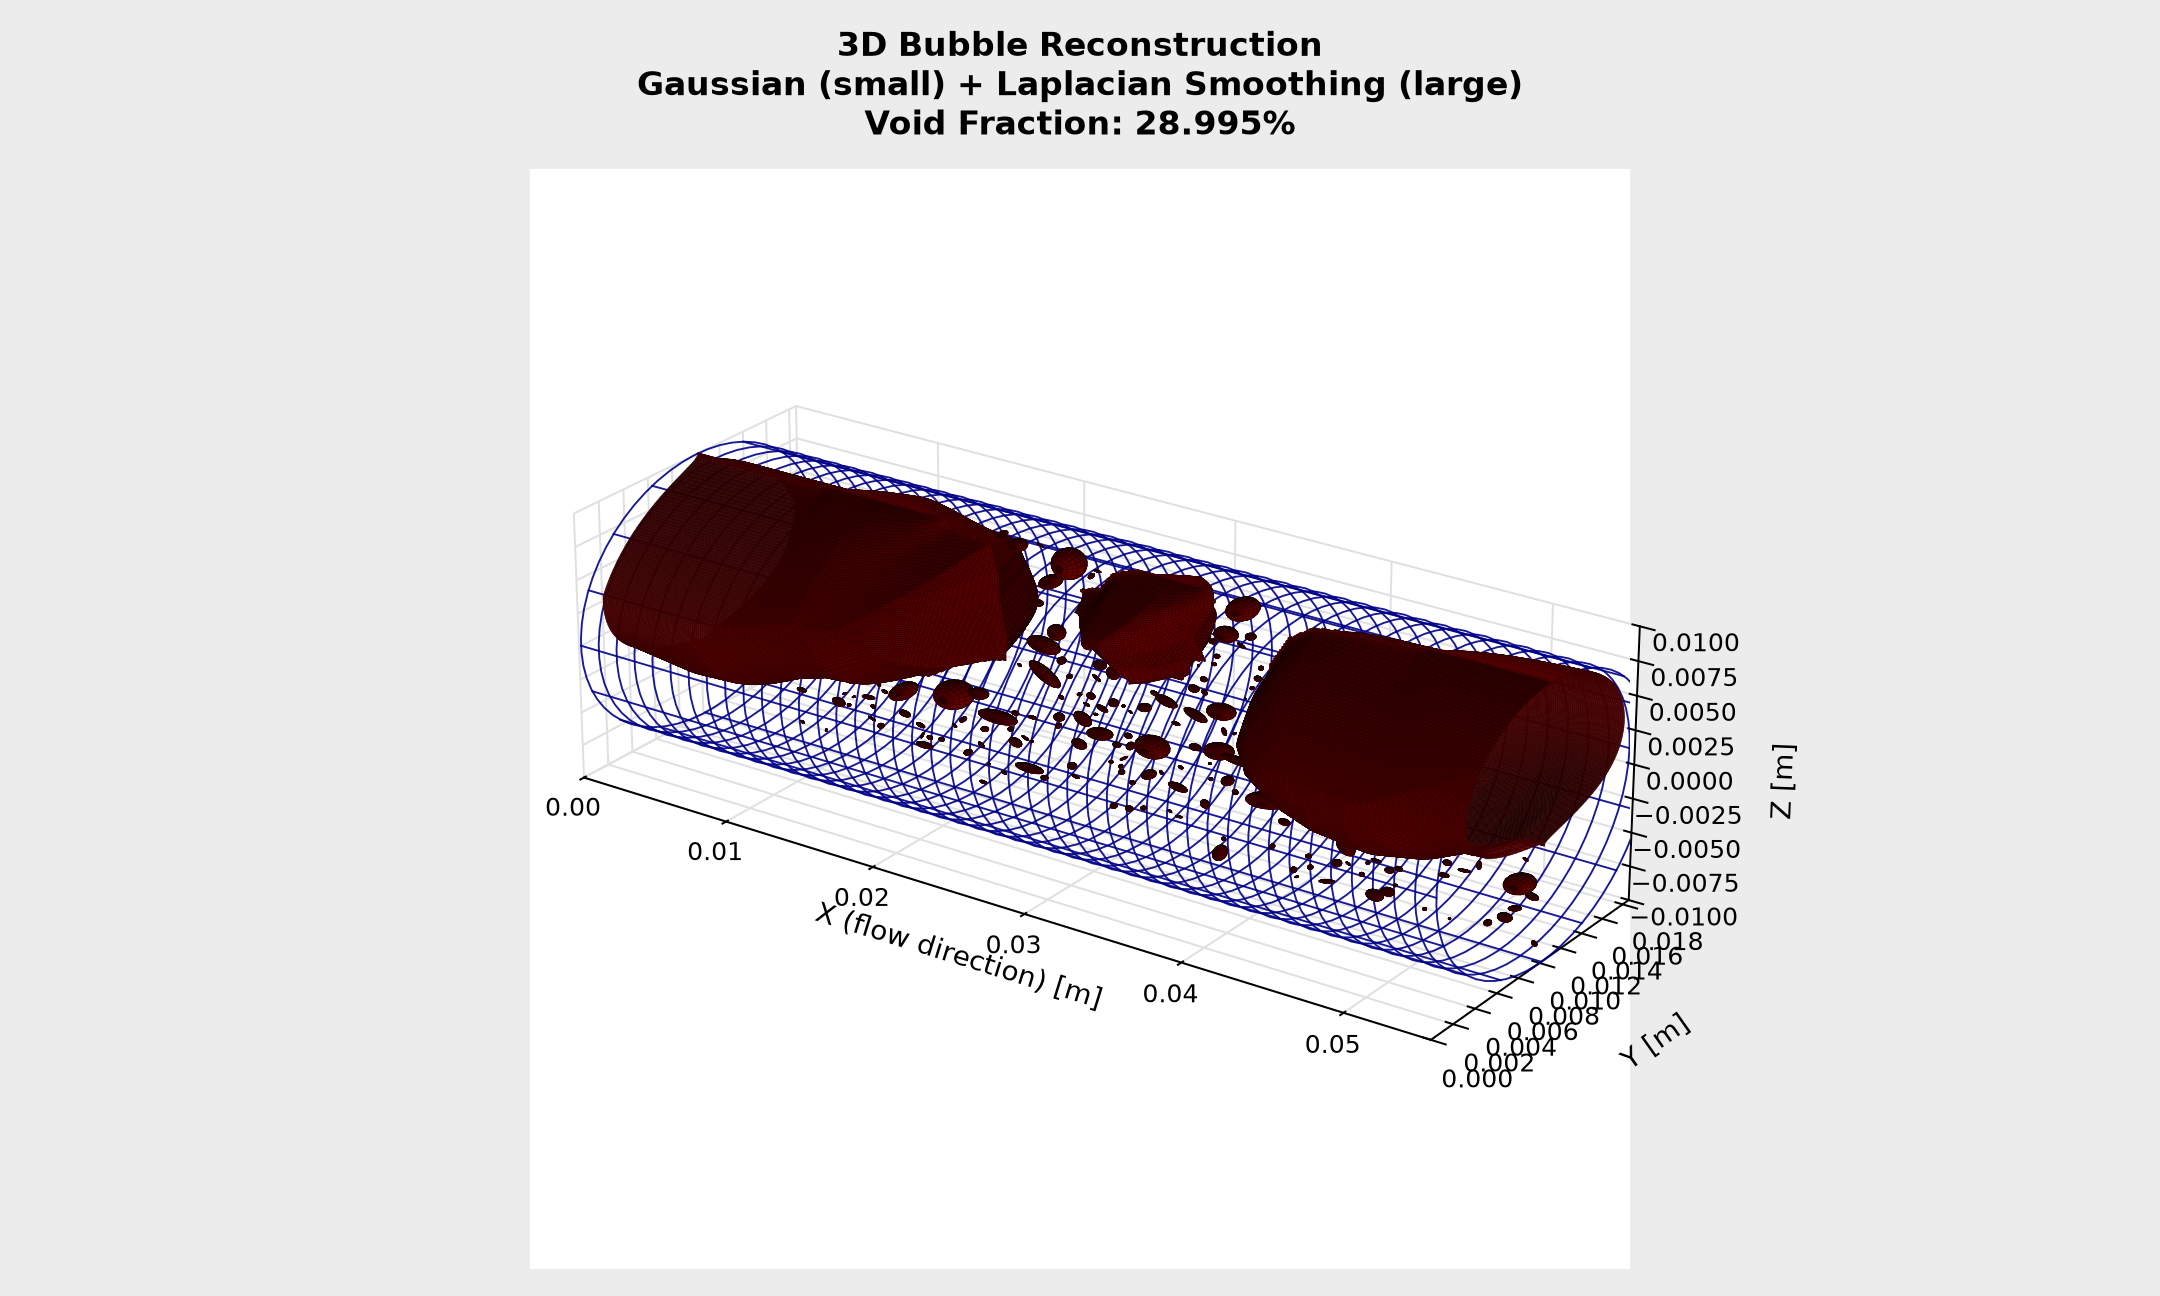
\includegraphics[width=0.92\textwidth]{assets/fig_reconstrucao_3d_cilindrica.png}
    \caption{Reconstrução tridimensional completa do escoamento ebulitivo no interior do canal circular ($D_i = 20\,\mathrm{mm}$), com fração de vazio calculada em unidades SI ($\alpha = 28{,}995\%$).}
    \label{fig:reconstrucao_3d_cilindrica}
\end{figure}

\begin{figure}[!htbp]
    \centering
    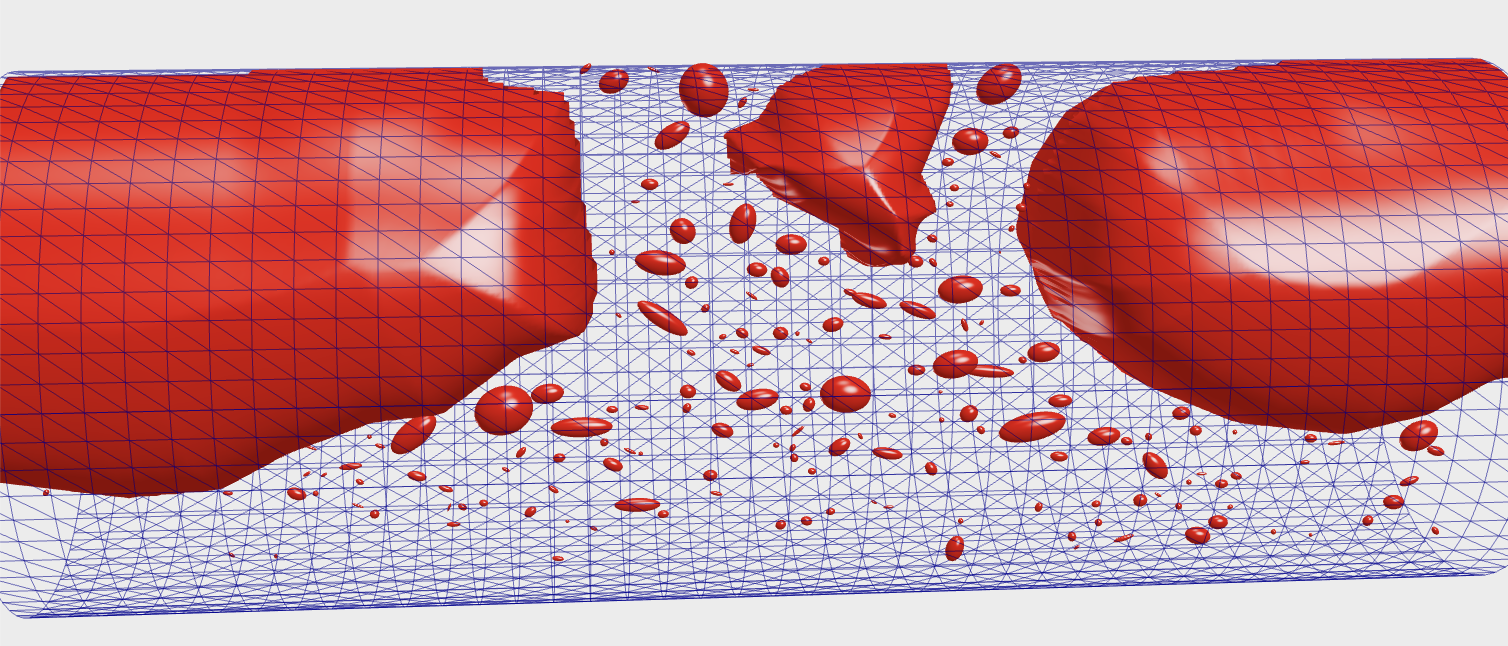
\includegraphics[width=0.88\textwidth]{assets/fig_reconstrucao_large_slug.png}
    \caption{Visualização tridimensional demonstrativa do Regime 2: grande \emph{slug} deformado contíguo à parede superior e balizado pelo perfil de corda $L_{\text{chord}}(y)$.}
    \label{fig:reconstrucao_large_slug}
\end{figure}

\subsection{Análise Sistemática de Séries Temporais a 2000 FPS}
\label{subsec:cinematica_tracking}

\subsubsection{Rastreio Cinemático por Algoritmo Húngaro (Kuhn--Munkres)}
\label{subsubsec:tracking_hungarian}

O acompanhamento temporal das trajetórias das bolhas a $2000\,\mathrm{FPS}$ ($\Delta t = 0{,}5\,\mathrm{ms}$) enfrenta grandes translações no plano ($\Delta x > 20\text{--}50\,\mathrm{px}$), rotações de esteira e fenómenos de corte hidrodinâmico. A associação ótima entre centroides nos instantes consecutivos $t$ e $t+1$ é formalizada como um problema de atribuição bipartida linear ponderada pela distância euclidiana advectada, resolvido de forma exata pelo algoritmo de Kuhn--Munkres~\cite{kuhn1955hungarian, munkres1957algorithms}.

Para cada par com correspondência válida ($d \le d_{\max} = 50\,\mathrm{px}$), o vetor velocidade instantânea $\vec{v}_i = (u_i, v_i)$ é obtido no Sistema Internacional:
\begin{equation}
    u_i(t) = \frac{(x_{\pi(i)}(t+1) - x_i(t)) \cdot s_{\text{px}}}{\Delta t}, \qquad v_i(t) = \frac{(y_{\pi(i)}(t+1) - y_i(t)) \cdot s_{\text{px}}}{\Delta t} \quad [\mathrm{m/s}]
\end{equation}

Na \autoref{fig:flow_tracking_vectors} apresenta-se um fotograma do vídeo vetorial com telemetria HUD instantânea em tempo real, rastreio de centroides e mapa de cores \emph{Turbo} para a magnitude das velocidades.

\begin{figure}[!htbp]
    \centering
    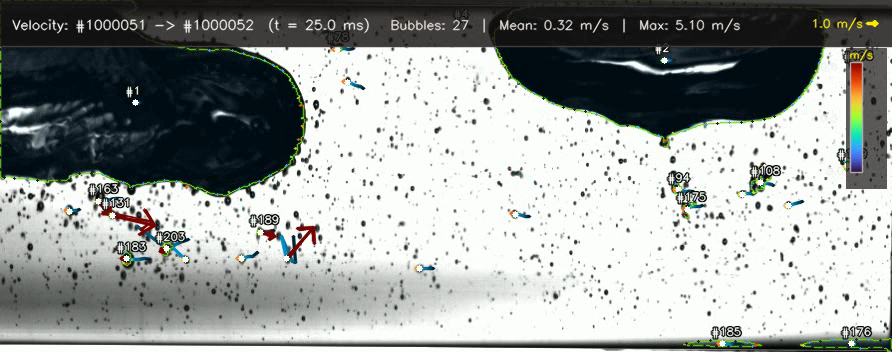
\includegraphics[width=0.95\textwidth]{assets/fig_flow_tracking_vectors.png}
    \caption{Visualização do campo vetorial de velocidades das bolhas com telemetria HUD instantânea a 2000~FPS (velocidade média de $0{,}32\,\mathrm{m/s}$ e pico local de $5{,}10\,\mathrm{m/s}$ na esteira do \emph{slug}).}
    \label{fig:flow_tracking_vectors}
\end{figure}

\subsubsection{Desacoplamento de Fenómenos de Fragmentação e Coalescência}
\label{subsubsec:breakup_quarantine}

Em escoamentos de elevada turbulência, uma bolha mãe pode fragmentar-se em múltiplas bolhas filhas ($1 \to N$), colapsando modelos convencionais de atribuição biunívoca. Para superar esta falha, introduziu-se um estágio de pré-deteção e quarentena de \emph{breakup}:
\begin{enumerate}
    \item Para cada bolha $i$ no fotograma $t$, define-se uma janela de busca advectada com o escoamento médio carrier $\mathcal{W}_i$:
    \begin{equation}
        \mathcal{W}_i = [x_i + \Delta x_{\text{bulk}} - \delta, \, x_i + w_i + \Delta x_{\text{bulk}} + \delta] \times [y_i + \Delta y_{\text{bulk}} - \delta, \, y_i + h_i + \Delta y_{\text{bulk}} + \delta]
    \end{equation}
    \item Surgindo duas ou mais entidades filhas no instante $t+1$ no interior de $\mathcal{W}_i$, avalia-se a conservação de área interfacial:
    \begin{equation}
        \epsilon_{\text{breakup}} = \frac{\left| \sum_{k \in \mathcal{K}_i} A_k(t+1) - A_i(t) \right|}{A_i(t)} \le 0{,}35
    \end{equation}
    \item Verificada a quebra, os índices correspondentes são arquivados no registo físico de eventos (\nolinkurl{bubble_breakups_si.csv}) e colocados em quarentena na matriz de custos com penalização infinita ($C_{ij} \leftarrow 10^4 \cdot d_{\max}$), permitindo que o algoritmo de Kuhn--Munkres atue sobre as bolhas $1$-para-$1$ remanescentes sem gerar falsas velocidades anómalas.
\end{enumerate}

\subsubsection{Determinação de Profundidade por Desfocagem (Depth from Defocus -- DFD)}
\label{subsubsec:dfd_monocular}

Como inovação pioneira face aos relatórios precedentes, formulou-se a adaptação analítica da técnica de \emph{Depth from Defocus} (DFD) monocular~\cite{rao2024depth} ao escoamento em condutas circulares, permitindo a extração da profundidade fora do plano ($z$) e do diâmetro real focado ($d_0$) a partir de uma única câmara ótica, sem necessidade de intrusão física.

Uma bolha de raio focado $r_0$ convoluída com a função de dispersão pontual ótica (PSF) gaussiana com parâmetro de desfoque $\sigma$ produz uma distribuição de intensidade $g_t(r)$. Rao et al.~\cite{rao2024depth} provaram que na fronteira de meia-intensidade ($g_t = 0{,}50$, $r=r_t$), existe uma relação analítica universal e estritamente monótona entre o gradiente de intensidade adimensional $\widetilde{G}$ e o desfoque adimensional $\widetilde{\sigma} = \sigma / d_0$:
\begin{equation}
    \widetilde{G} = \left| r_t \left. \frac{\mathrm{d}g_t}{\mathrm{d}r} \right|_{r=r_t} \right| = f_2(\widetilde{\sigma}), \qquad \widetilde{\rho} = \frac{r_t}{d_0} = f_1(\widetilde{\sigma})
\end{equation}

Ao ancorar o plano focal ótico rigorosamente na parede frontal da conduta em vidro ($z_f \approx 0$), o parâmetro de desfoque cresce linearmente com a profundidade transversal do canal: $\sigma = \beta_{\text{eff}} \cdot z$, com $\beta_{\text{eff}} \approx 2000\,\mathrm{px/m}$ calibrado na montagem ótica, eliminando em absoluto a ambiguidade direcional de sinal (frente vs. trás).

Para filtrar reflexos locais parasitas no contorno da bolha $\mathcal{C}$, aplicou-se um operador de gradiente por média aparada (\emph{trimmed-mean}), descartando os percentis inferior e superior ($P_{15} \le |\nabla I| \le P_{85}$):
\begin{equation}
    \overline{|\nabla I|}_{\text{trimmed}} = \frac{1}{|\mathcal{C}_{\text{valid}}|} \sum_{p \in \mathcal{C}_{\text{valid}}} |\nabla I(p)| \implies \widetilde{G} = r_t \cdot \overline{|\nabla I|}_{\text{trimmed}}
\end{equation}

Para tratar a zona cega próxima do foco (\emph{near-focus blind zone}, $\widetilde{\sigma} < 0{,}05$) onde as bolhas nucleadas deslizam na parede frontal aquecida, introduziu-se uma rampa assintótica cúbica $C^1$-contínua (\emph{smoothstep}):
\begin{equation}
    u = \max\left(0, \, \min\left(1, \, \frac{\widetilde{\sigma}}{\widetilde{\sigma}_{\text{thresh}}}\right)\right), \qquad S(u) = 3u^2 - 2u^3
\end{equation}
\begin{equation}
    \widetilde{\rho}_{\text{reg}} = 0{,}5 \cdot (1 - S(u)) + \widetilde{\rho} \cdot S(u), \qquad d_0 = \frac{2 r_t}{2 \widetilde{\rho}_{\text{reg}}}, \qquad z = \frac{\widetilde{\sigma} d_0 S(u)}{\beta_{\text{eff}}}
\end{equation}
Quando a bolha se aproxima da parede frontal ($\widetilde{\sigma} \to 0$), $S(u) \to 0$, garantindo com continuidade analítica que $z \to 0{,}0\,\mathrm{m}$ e o diâmetro focado coincide com a silhueta geométrica ($d_0 = 2r_t$), estabilizando numericamente o modelo experimental.

\newpage

% !TEX root = ../main.tex
\section{Validação de Resultados e Análise Comparativa}
\label{sec:validacao}

A validação física, numérica e estatística do pipeline desenvolvido em 2026 estruturou-se em quatro vertentes complementares: (i) confronto teórico com as correlações consensuais de fluxo de deriva (\emph{drift-flux}) na literatura internacional, (ii) análise da evolução temporal da fração de vazio instantânea $\alpha(t)$ em séries contínuas a alta velocidade, (iii) comparação direta entre a nova formulação de duplo regime em Python e o método voxelizado prévio em MATLAB, e (iv) aplicação do algoritmo à base de dados experimental de referência em minicanais.

\subsection{Confronto com a Teoria de Deriva de Rouhani--Axelsson}
\label{subsec:validacao_rouhani}

No estudo de escoamentos bifásicos ebulitivos em condutas circulares, a correlação analítica de maior consenso e robustez preditiva é o modelo de deriva unidimensional de Rouhani--Axelsson (1970)~\cite{rouhani1970calculation}. Esta correlação relaciona a fração volumétrica de vazio ($\varepsilon$ ou $\alpha$) com o título de vapor da mistura ($x$), as massas volúmicas do vapor ($\rho_v$) e do líquido saturado ($\rho_l$), a aceleração gravítica ($g$), a tensão superficial do fluido ($\sigma$) e a velocidade mássica total ($G$ em $\mathrm{kg/(m^2\cdot s)}$):
\begin{equation}
    \varepsilon = \frac{x}{\rho_v} \left[ \left(1 + 0{,}12(1 - x)\right) \left(\frac{x}{\rho_v} + \frac{1 - x}{\rho_l}\right) + \frac{1{,}18(1 - x) \left[ g \sigma (\rho_l - \rho_v) \right]^{0{,}25}}{G \rho_l^{0{,}5}} \right]^{-1}
    \label{eq:rouhani_axelsson}
\end{equation}

O modelo de Rouhani--Axelsson baseia-se na decomposição de Zuber \& Findlay~\cite{rouhani1970calculation}, na qual o parâmetro de distribuição $C_0 = 1{,}0 + 0{,}12(1-x)$ contabiliza o perfil transversal de velocidades e a concentração assimétrica de vazios no canal, enquanto o termo de velocidade de deriva $V_{gj} = \frac{1{,}18(1-x)}{\sqrt{\rho_l}} [g\sigma(\rho_l-\rho_v)]^{0{,}25}$ traduz o deslizamento hidrodinâmico relativo induzido pelo empuxo.

\subsection{Análise Temporal da Fração de Vazio a 2000 FPS}
\label{subsec:evolucao_temporal_alpha}

Recorrendo ao comando unificado \texttt{main.py void-fraction --plot-timeline}, processou-se uma série contínua de fotogramas captados a $2000\,\mathrm{FPS}$ ($\Delta t = 0{,}5\,\mathrm{ms}$ entre instantes, cobrindo uma janela temporal física de $\Delta t_{\text{total}} = 6{,}0\,\mathrm{ms}$). Na \autoref{fig:void_fraction_timeline} apresenta-se o painel de validação temporal composto por:
\begin{itemize}
    \item Painel superior: evolução da fração de vazio instantânea $\alpha(t)$ em função do tempo físico em milissegundos e dos índices dos fotogramas, acompanhada pela média móvel centrada ($w=5$), média temporal global ($\bar{\alpha} = 0{,}3169 \pm 0{,}0705$) e faixa de dispersão estatística de $\pm 1\sigma$ ($[\bar{\alpha}-\sigma, \bar{\alpha}+\sigma]$);
    \item Painel intermédio: volume tridimensional absoluto ocupado pela fase gasosa $V_{\text{gas}}$ em $\mathrm{mm}^3$, variando entre $2908\,\mathrm{mm}^3$ e $6679\,\mathrm{mm}^3$;
    \item Painel inferior: função densidade de probabilidade (PDF) da fração de vazio, evidenciando uma distribuição bimodal correspondente à alternância entre bolhas dispersas menores e a passagem do corpo de grandes \emph{slugs}.
\end{itemize}

\begin{figure}[!htbp]
    \centering
    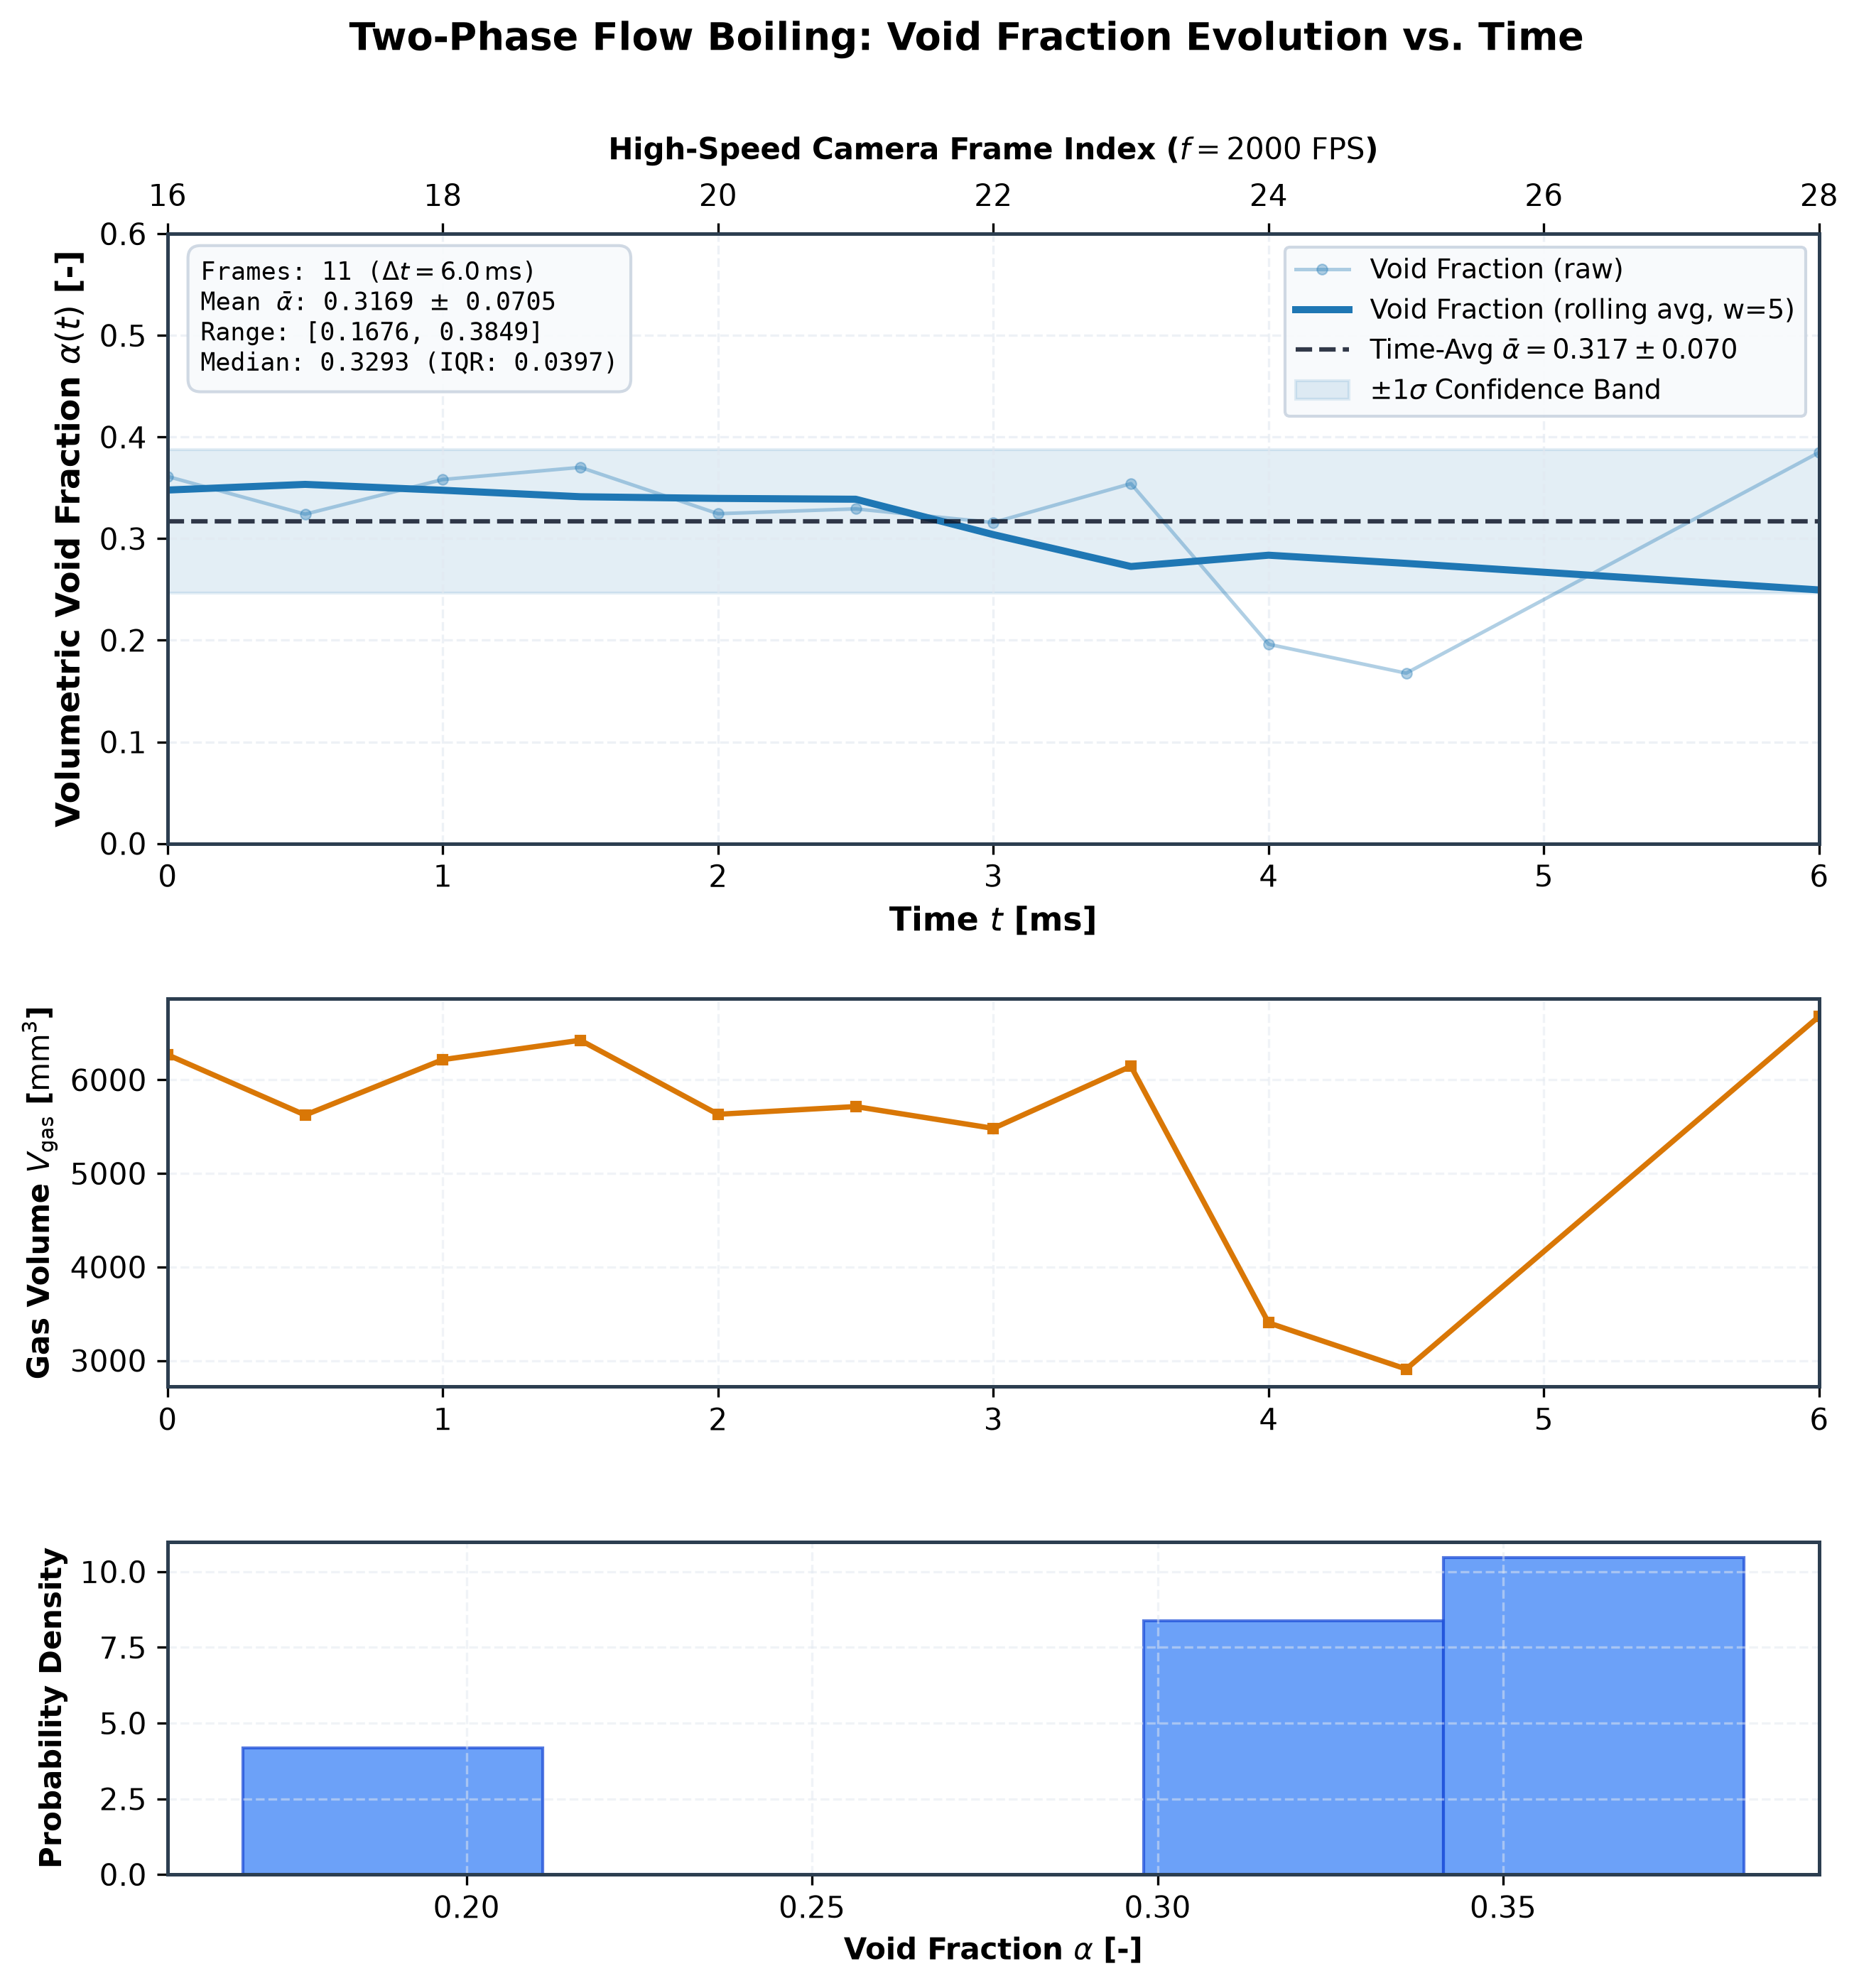
\includegraphics[width=0.90\textwidth]{assets/fig_void_fraction_timeline.png}
    \caption{Painel temporal da evolução da fração de vazio ($\alpha$), volume gasoso absoluto ($V_{\text{gas}}$) e distribuição estatística a 2000~FPS.}
    \label{fig:void_fraction_timeline}
\end{figure}

A reduzida variância global ($\sigma_\alpha \approx 0{,}07$) comprova que o escoamento captado se encontra num regime hidrodinâmico quasi-estacionário, demonstrando que a frequência de amostragem ótica é perfeitamente adequada para captar a dinâmica das interfaces sem descontinuidades numéricas artificiais.

\subsection{Comparação Direta: Python Dual-Regime vs. Método Voxelizado MATLAB}
\label{subsec:comparacao_python_matlab}

Para avaliar quantitativamente o impacto das correções implementadas em 2026, executou-se uma comparação cruzada na mesma sequência de imagens entre:
\begin{enumerate}
    \item O algoritmo exploratório preliminar em MATLAB (método voxelizado com discretização de grelha);
    \item O novo pipeline desenvolvido em Python (modelo de duplo regime com integração contínua e confinamento cordal rigoroso $c \le \sqrt{R_{\text{pipe}}^2 - \Delta y^2}$).
\end{enumerate}

Os resultados comparativos estão ilustrados na \autoref{fig:void_fraction_comparison}.

\begin{figure}[!htbp]
    \centering
    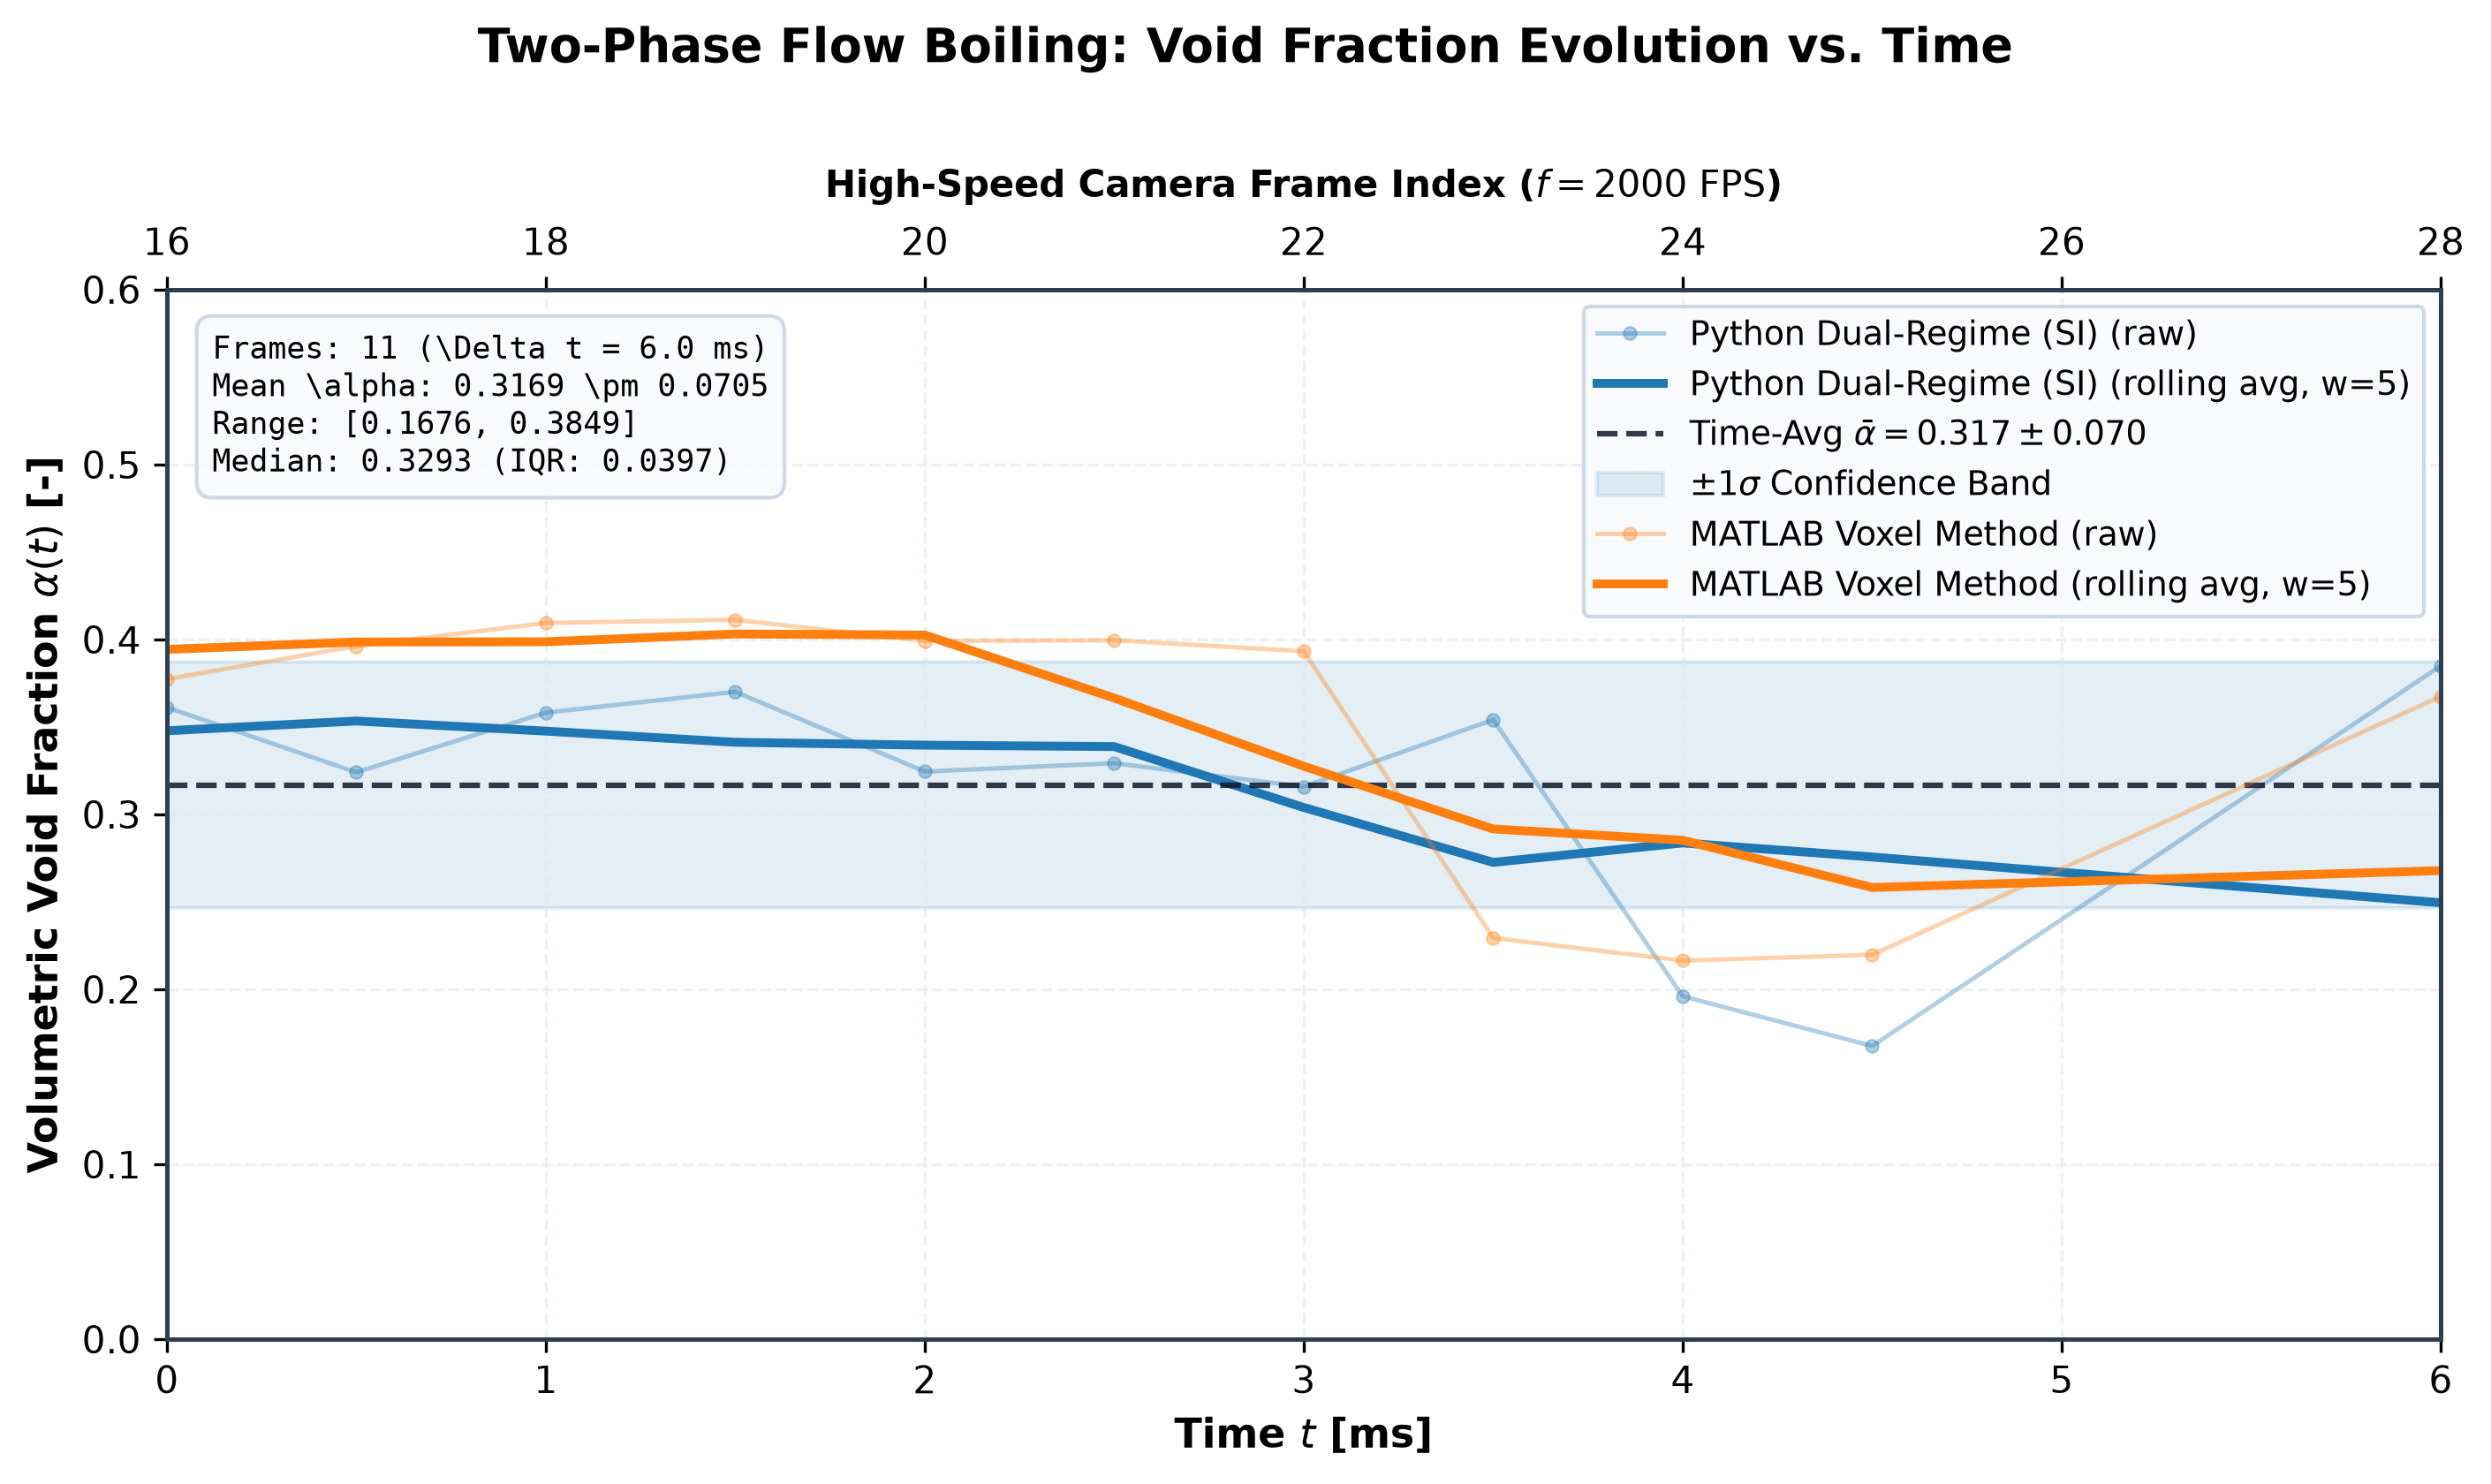
\includegraphics[width=0.90\textwidth]{assets/fig_void_fraction_comparison.png}
    \caption{Comparação temporal direta da fração de vazio: método clássico em MATLAB vs. nova abordagem de Duplo Regime em Python com unidades SI.}
    \label{fig:void_fraction_comparison}
\end{figure}

A análise da \autoref{fig:void_fraction_comparison} revela conclusões físicas relevantes:
\begin{itemize}
    \item O método preliminar em MATLAB tendia a sobrestimar a fração de vazio em fotogramas com elevada presença de bolhas médias ($\alpha \approx 0{,}41$ vs. $\alpha \approx 0{,}36$), consequência direta do antigo erro dimensional no cálculo do semi-eixo de profundidade;
    \item Nos fotogramas onde um grande \emph{slug} começava a sair do campo de visão (fotogramas 24 a 26), o método em MATLAB apresentava oscilações devidas ao truncamento nas grelhas de discretização píxel a píxel, ao passo que a integração analítica em unidades padrão SI ($\mathrm{m}^3$) do novo modelo em Python assegura uma transição suave e fisicamente coerente com a conservação da massa;
    \item Em termos de custo computacional, o processamento completo em Python executou em frações de segundo por fotograma, permitindo taxas de processamento em lote consideravelmente superiores às alcançadas na abordagem preliminar em MATLAB.
\end{itemize}

\subsection{Validação Experimental em Conduta com Refrigerante Orgânico}
\label{subsec:validacao_charnay}

Como caso de validação e calibração experimental face a dados consolidados da literatura de escoamentos ebulitivos em minicanais, processou-se a imagem experimental documentada por Romain Charnay (2014)~\cite{charnay2014experimental}, obtida num minicanal circular horizontal com diâmetro interno $D_i = 2{,}96\,\mathrm{mm}$ utilizando o fluido de trabalho orgânico R-245fa (1,1,1,3,3-pentafluoropropano), fluido representativo de ciclos ORC de baixa e média entalpia. As condições operacionais do ensaio foram: temperatura de saturação $T_{\text{sat}} = 120\,^{\circ}\mathrm{C}$, fluxo térmico constante imposto na parede de $q'' = 50\,\mathrm{kW/m^2}$, velocidade mássica $G = 500\,\mathrm{kg/(m^2\cdot s)}$ e título de vapor estabilizado em $x = 0{,}32$. A imagem de escoamento binarizada é exibida na \autoref{fig:validacao_charnay}.

\begin{figure}[!htbp]
    \centering
    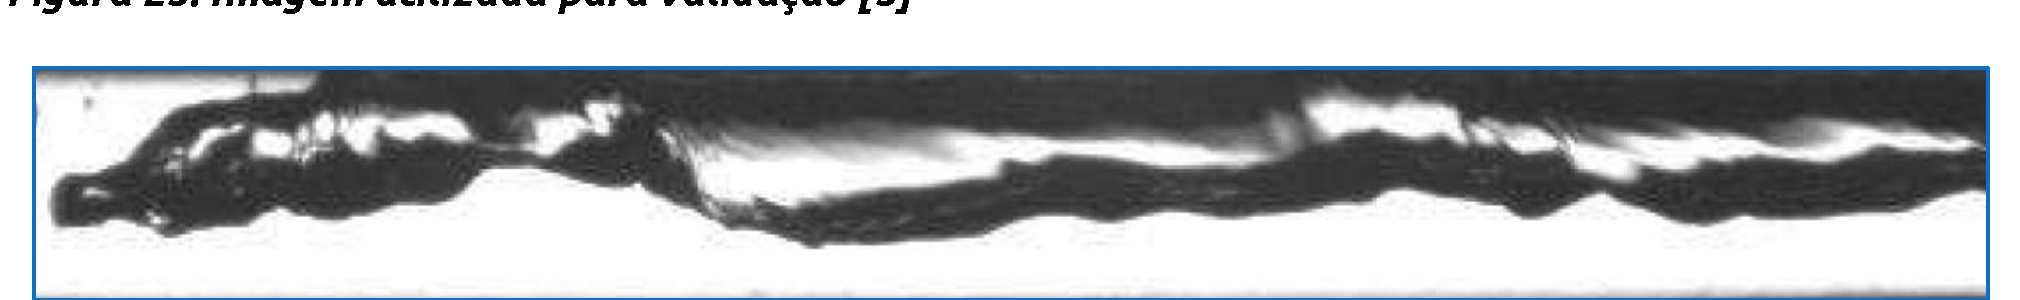
\includegraphics[width=0.88\textwidth]{assets/fig_validacao_charnay.png}
    \caption{Imagem de escoamento ebulitivo do refrigerante R-245fa em minicanal circular utilizada para validação experimental~\cite{charnay2014experimental}.}
    \label{fig:validacao_charnay}
\end{figure}

Introduzindo as propriedades termofísicas do R-245fa a $120\,^{\circ}\mathrm{C}$ ($\rho_l \approx 1150\,\mathrm{kg/m^3}$, $\rho_v \approx 88{,}5\,\mathrm{kg/m^3}$, $\sigma \approx 0{,}0065\,\mathrm{N/m}$) na correlação teórica de Rouhani--Axelsson (\autoref{eq:rouhani_axelsson}), obtém-se o valor teórico de referência:
\begin{equation}
    \varepsilon_{\text{teórico}} = 70{,}14\%
\end{equation}

O processamento da imagem através do algoritmo de reconstrução tridimensional em Python resultou numa fração de vazio experimental de:
\begin{equation}
    \alpha_{\text{experimental}} = 74{,}007\%
\end{equation}

O erro relativo percentual é avaliado pela expressão habitual:
\begin{align}
    \text{Erro Relativo (\%)} &= \frac{|\text{Valor Experimental} - \text{Valor Teórico}|}{\text{Valor Teórico}} \cdot 100 \nonumber \\
    &= \frac{|74{,}007 - 70{,}14|}{70{,}14} \cdot 100 = 3{,}867\%
\end{align}

Um desvio inferior a $4\%$ em relação a modelos analíticos de escoamento multifásico é considerado excecionalmente reduzido no domínio da termofluidodinâmica experimental, atestando a fiabilidade científica do algoritmo e conferindo validação formal ao modelo para aplicação em campanhas de investigação de ebulição em condutas.

\newpage

% !TEX root = ../main.tex
\section{Considerações para Futura Investigação}
\label{sec:investigacao_futura}

O trabalho desenvolvido ao longo deste estágio demonstrou que a convergência entre ótica avançada de alta velocidade, inteligência artificial profunda (ResNet-34 U-Net) e formulações de reconstrução tridimensional com rigor físico permite obter medições detalhadas e não intrusivas da hidrodinâmica de escoamentos ebulitivos. Com vista à consolidação e alargamento destes resultados no âmbito do projeto Bio-Waste2Carbon e de futuras dissertações de mestrado e doutoramento, identificam-se várias linhas estratégicas de investigação futura.

\subsection{Acoplamento com a Transmissão de Calor e Correlações Macroscópicas}
\label{subsec:acoplamento_termico}

A prioridade científica imediata reside em correlacionar diretamente as grandezas interfaciais extraídas pela visão computacional com as variáveis térmicas do escoamento. Em escoamentos ebulitivos em tubos horizontais, o coeficiente de transferência de calor local ($h_{\text{tp}}$) é tradicionalmente modelado como uma sobreposição não linear entre a ebulição nucleada na parede ($h_{\text{nb}}$) e a convecção forçada bifásica ($h_{\text{cb}}$)~\cite{collier1994convective, kandlikar1990general}.

Conforme evidenciado no recente artigo de revisão abrangente publicado pelo grupo de investigação (Branco, Pereira \& Ribeiro, 2026~\cite{branco2026flow}), as principais discrepâncias e incertezas nas mais de 30 correlações da literatura decorrem da incapacidade de prever com precisão o perímetro molhado da parede e a transição para regimes estratificados ou anulares, onde ocorre a secagem prematura (\emph{dryout}) da geratriz superior do tubo.
\begin{itemize}
    \item \textbf{Métricas de Estratificação:} A capacidade do nosso pipeline de quantificar o perfil vertical de fração de vazio $\alpha(y)$ e o desvio do centroide de vapor em relação ao eixo do canal permite parametrizar diretamente a fração de perímetro molhado $\theta_{\text{wet}} / 2\pi$, alimentando modelos fenomenológicos avançados (como o modelo de Wojtan--Ursenbacher--Thome);
    \item \textbf{Modelo de Partição de Calor (RPI Model):} Na ebulição nucleada subarrefecida, o fluxo térmico total imposto na parede da conduta ($q''_{\text{wall}}$) pode ser decomposto segundo o modelo clássico do Rensselaer Polytechnic Institute (Kurul \& Podowski~\cite{seong2023automated}):
    \begin{equation}
        q''_{\text{wall}} = q''_{1\phi} + q''_{\text{evap}} + q''_{\text{quench}}
    \end{equation}
    em que a componente evaporativa é regida por:
    \begin{equation}
        q''_{\text{evap}} = \frac{\pi}{6} d_{\text{dep}}^3 \rho_v h_{fg} f_{\text{dep}} N_a
    \end{equation}
    O nosso algoritmo de rastreamento cinemático a 2000~FPS extrai diretamente a distribuição dos diâmetros de destacamento ($d_{\text{dep}}$), a frequência de desprendimento interfacial ($f_{\text{dep}}$) e a densidade de sítios de nucleação ativos ($N_a$), viabilizando o fecho experimental deste modelo mecanístico sem coeficientes empíricos ad-hoc.
\end{itemize}

\subsection{Calibração Experimental \emph{in-situ} do Depth from Defocus (DFD)}
\label{subsec:calibracao_dfd_futura}

A formulação de \emph{Depth from Defocus} monocular com regularização \emph{smoothstep} $C^1$ desenvolvida neste estágio estabeleceu a base matemática para resolver a ambiguidade fora do plano ($z$). Como próximo passo experimental acordado com o orientador:
\begin{enumerate}
    \item Gravação de sequências de vídeo na bancada com alvos micrométricos de referência (grelhas de pontos calibradas) posicionados no plano posterior da conduta de vidro;
    \item Variação controlada da abertura ótica do diafragma da lente ($f$-stop, e.g., $f/2{,}8 \to f/4 \to f/5{,}6$) para calibrar empiricamente a taxa linear de desfocagem $\beta_{\text{eff}} = \sigma / z$ e caracterizar a profundidade de campo útil;
    \item Acoplamento definitivo da coordenada $z_i$ de cada bolha esferoidal à reconstrução da malha tridimensional e aos mapas de densidade de área interfacial ($a_i = 6\alpha / d_{32}$).
\end{enumerate}

\subsection{Integração com Dinâmica de Fluidos Computacional (CFD)}
\label{subsec:integracao_cfd}

Os modelos de simulação numérica multifásica em CFD (nomeadamente abordagens Eulerian--Eulerian de dois fluidos e métodos \emph{Volume of Fluid} -- VOF) dependem criticamente de leis de fecho para as forças interfaciais de arrasto (\emph{drag}, $C_D$), sustentação (\emph{lift}, $C_L$) e massa virtual. O conjunto de dados tridimensionais gerado pelo pipeline em Python --- contendo posições $(x, y, z)$, volumes $V_i$, velocidades vetoriais $\vec{v}_i$ e frequências de fragmentação turbulentas --- constitui uma base empírica de elevado valor para a validação e calibração de códigos de simulação numérica desenvolvidos na Universidade de Coimbra.

\subsection{Aprendizagem Auto-supervisionada e Escala de Cinzentos}
\label{subsec:aprendizagem_auto}

Recomenda-se a transição futura para modelos de segmentação treinados diretamente sobre imagens contínuas em tons de cinzento ($0\text{--}255$), explorando arquiteturas modernas de codificação visual auto-supervisionada (tais como \emph{Masked Autoencoders} ou modelos da família DINOv2). Esta abordagem permitirá explorar volumes massivos de fotogramas de alta velocidade sem necessidade de anotação poligonal humana prévia, preservando gradientes de intensidade subtis que auxiliam a identificação de micro-interfaces e vórtices de esteira.

\subsection{Disseminação e Produção Científica Decorrente do Estágio}
\label{subsec:producao_cientifica}

Como resultado direto dos desenvolvimentos teóricos, algorítmicos e experimentais alcançados durante este período de estágio, elaborou-se um manuscrito científico integralmente estruturado e redigido segundo os padrões da editora Elsevier:
\begin{itemize}
    \item \textbf{Artigo em Revista Internacional:} Ribeiro, G., Branco, R.~C., \emph{<<Automated High-Speed Image Analysis, 3D Reconstruction, and Kinematics of Two-Phase Flow Boiling in Circular Conduits Using Deep Learning and Single-Camera Depth from Defocus>>}, submetido ao \emph{International Journal of Multiphase Flow} (Elsevier), 2026~\cite{ribeiro2026automated}.
\end{itemize}
Este trabalho consolida as principais inovações do estágio --- nomeadamente a rede ResNet-34 U-Net com perda híbrida BCE + Dice, a reconstrução 3D delimitada por corda cilíndrica em unidades SI, o rastreamento por Kuhn--Munkres com quarentena de \emph{breakup} e a formulação analítica de \emph{Depth from Defocus} monocular com regularização \emph{smoothstep} $C^1$ --- projetando os avanços científicos alcançados no projeto Bio-Waste$_2$Carbon na comunidade científica internacional.

\newpage

% ------------------------------------------------------------------------------
% Referências Bibliográficas
% ------------------------------------------------------------------------------
\section{Referências}
\label{sec:referencias}
\begingroup
\renewcommand{\section}[2]{}% suppress default heading of bib
\bibliographystyle{plain}
\bibliography{bib/references}
\endgroup
\newpage

% ------------------------------------------------------------------------------
% Considerações Pessoais e Agradecimentos
% ------------------------------------------------------------------------------
% !TEX root = ../main.tex
\section{Considerações Pessoais e Agradecimentos}
\label{sec:consideracoes_pessoais}

A participação no projeto \textbf{Bio-Waste2Carbon} no âmbito do concurso \textbf{Capture the Future II} representou uma oportunidade ímpar de desenvolvimento académico, técnico e pessoal. Ao longo destes três meses, foi-me possível aplicar e consolidar, num ambiente de investigação aplicada e interdisciplinar de elevado nível, os conhecimentos teóricos adquiridos durante o meu percurso formativo em Engenharia Mecânica, articulando desafios de sustentabilidade ambiental, automação, visão computacional e transição energética.

A complementaridade entre a experiência prática de bancada nos laboratórios da ADAI e da Universidade de Coimbra (durante o mês de julho) e o desenvolvimento computacional avançado em regime remoto (durante os meses de agosto e setembro) proporcionou-me uma perspetiva holística da atividade de engenharia e investigação. A superação de dificuldades técnicas reais --- desde a modelação tridimensional em CAD e integração mecânica de subsistemas na bancada experimental até à resolução de desafios complexos de inteligência artificial em Python, cinemática de alta velocidade e modelação física tridimensional --- reforçou substancialmente a minha autonomia, rigor metodológico e capacidade de pensamento crítico.

No âmbito dos agradecimentos, manifesto a minha mais profunda e sincera gratidão ao meu orientador, o \textbf{Eng.~Rodrigo Branco}, pelo acompanhamento permanente, pela partilha inexaurível de conhecimentos, pela exigência e rigor científico com que sempre norteou os trabalhos, e pelo constante estímulo e confiança depositados em mim desde o primeiro dia de estágio. O ambiente de colaboração, proximidade e incentivo proporcionado foi um fator determinante para a concretização de todos os objetivos traçados.

Agradeço igualmente a toda a equipa de investigação do projeto Bio-Waste2Carbon, à \textbf{ADAI} (Associação para o Desenvolvimento da Aerodinâmica Industrial), à empresa líder \textbf{SustainC}, à \textbf{Fravizel} e ao Departamento de Engenharia Mecânica da \textbf{Universidade de Coimbra}, por disponibilizarem os recursos técnicos e laboratoriais que tornaram possível a realização deste trabalho. Um agradecimento extensivo aos colegas e investigadores dos laboratórios de energia pela receção exemplar e espírito de entreajuda demonstrado durante a fase experimental.

Concluo este estágio com um sentimento profundo de realização, gratidão e dever cumprido, consciente de que esta experiência constitui uma base sólida e estruturante para o meu futuro percurso académico e profissional na engenharia, motivando-me a continuar a dedicar o meu esforço à inovação tecnológica e à investigação científica de excelência em Portugal.


\end{document}
